\def\fr{30}
\def\edg{边缘服务端}
\def\fr{10}
\def\acc{72.7\%}
\def\idenT{93毫秒}
\def\uiT{20秒}

\chapter{引言}
\label{chap:introduction}
近年来,物联网(IoT)产业发展迅速。根据相关机构的预测\cite{macgillivray2019worldwide},2025年将安装820亿台物联网设备。因此,人们将会与越来越多的设备进行交互。由于成本原因,物联网设备一般很少具有人可以操作的物理接口,一般最多会安装按钮或开关。因此物联网领域中最为主流的交互形式是使用应用程序通过一个智能设备(如手机或笔记本电脑)来控制物联网设备\cite{homeass,xiaomi}。此外,家庭生活中也越来越流行安装智能音箱并通过语音命令对家居设备进行交互\cite{li2019iot,porcheron2018voice}。与上述人机交互形式相比,增强现实(AR)技术能够直接在设备本体上显示出设备的信息和交互界面,可以打破物理空间和数字空间之间的界限,实现所见即所得。

在行业中,最主流的交互形式是使用一个手机应用程序(APP)来控制一组设备。这种方式的优点是无须为设备提供多余的实体操作面板,可以降低设备成本,同时也可以通过一台手机控制多个设备。缺点是,这种情况下大量同类设备的管理会给用户带来麻烦,用户必须自己链接物理空间和数字空间,也就是说,如果他们想要控制特定的设备,他们必须首先在应用程序的设备列表中找到相应的项目,并确定该项目所对应的设备正是自己面前想要操作的设备。

另一种新兴的交互式方法是语音交互。谷歌、亚马逊和苹果都设计并上市了他们的智能音箱\cite{googlehome,AmazonEcho,apple-homepod},这些智能音箱可以通过WiFi等方式连接到家庭中所有可连接的设备。语音交互的优点是它在一定程度上减轻了用户的操作负担,因为他们只需说出自己的请求,而无需指明所要操作的设备。
然而,当交互目的变得复杂时,比如家中安装了两台相同型号的设备时,基于语音的交互同样会遇到物理与数字空间如何直观链接的问题。

Google Physical Web\cite{jenson2014physical}为设备发现提供了一种更加自动化的方式:它把虚拟的Web延伸到周围的物理世界,目标是新开发出一套可以供所有设备共同支持的Web标准,以便让任何设备都可以以此为标准,向用户提供交互以及一系列对应的设备服务。利用这套标准,智能设备可以通过低功耗蓝牙协议把自己的URL地址广播给周围,周围的任何设备(如智能手机、平板电脑)可以接收到这些URL然后呈现给用户。用户随后就可以根据需要通过URL与这些设备直接交互而不需要下载APP。但它同样没有解决设备的链接问题,手机里显示出周围的设备的URL后,用户仍然无法确定具体的物理设备和URL之间的联系。

学术界在这方面做了一些工作,尝试用先进技术填补将物理空间和数字空间链接的空白。
QR码是日常生活中非常常见的技术,目前能达到很高的识别成功率,但是基于QR码的解决方案会受到观察距离和观察角度的限制,同时QR码需要改造设备外观。还有一些工作\cite{alanwar2017selecon}在每个设备上部署传感节点以对外广播自己得到设备ID,如UWB或RFID标签,这需要改造现有的物联网设备,为其加上额外的部件,需要比较高的成本。

现有的一些工作试图通过类似增强现实的设计实现人机交互\cite{de2016snap,chen2018snaplink}。Snap-To-It\cite{de2016snap}使得用户可以通过拍摄设备照片并发送到服务器来选定要操作的设备,如果照片与某个设备成功匹配,服务器将返回该设备的交互界面并在手机上显示。SnapLink\cite{chen2018snaplink} 没有在识别设备的时候同时识别设备在图片上的位置,但是也用同样方式实现了对设备的控制。然而,这两个工作只能在设备照片被拍摄后对该设备进行识别,速度不够快。Snap-To-It和Snap都证明了将计算机视觉引入物理空间和数字空间链接是非常有效的,能实现直观的交互,但这种方法仍然存在局限性。
在用户体验上,拍照动作限制了设备发现的速度,因为这要求用户按下快门并等待响应。想象一下,一个用户来到一个新的地方,他为了找出可以访问的对象,需要花费大量的时间和精力来拍摄环境中的物体。

增强现实技术完美地解决了物理空间和数字空间的链接问题,学术界也做很多基于增强现实技术的人机交互解决方案。比如有工作\cite{liu2019edge} 研究了边缘辅助的实时移动增强现实技术,实现了高速移动中的增强现实技术。但是对于人机交互来说,该方法仍然缺乏识别设备的能力。一些工作\cite{ben2020edge,xu2020edge,liu2021edgesharing}提出了边缘辅助的同步定位和地图构建(Simultaneous Localization and Mapping, SLAM),实现了真正的实时SLAM。它们已经可以用于实现基于增强现实的人机交互,但他们还需要进一步的集成工作,比如设备的识别,设备移动后地图的更新,如何与具体设备进行交互等问题。
从系统灵活性的角度来看,这些工作都缺乏用户定制交互体验的能力。
现有的实现大多需要开发人员设计交互界面,这使得系统的应用不够灵活。
对于用户来说,可以访问的设备、可以执行的交互操作和数据都是固定的,难以进行修改和定制。

本文认为实现基于增强现实的人机交互有三个要求:

1) 视频帧中的设备应被准确识别和定位,处理速度足够快,用户感觉不到延迟或掉帧;

2) 设备发生移动后地图随之动态更新,系统能适应物理空间的动态变化;

3) 交互操作以用户为导向,用户要有高质量交互体验。

此外,我们注意到一个有趣的现象,人们不仅希望与可连接的设备(即具有基本通信能力的设备)交互,而且希望与不可连接的对象进行交互。例如,对于一棵植物,用户可能希望能在植物物理空间对应的数字空间处记录自己培育植物的记录(例如每次浇水的时间和最近的浇水量)。因此,本文希望将可连接/不可连接的对象都视为交互目标,将人与设备的交互进一步转化为人与对象的交互。

为了解决增强现实交互方案的上述局限性,本文提出了VSLink,这是一种基于视觉SLAM和神经网络来连接物理和数字空间的方法,它在边缘端实现了快速的对象定位与识别,地图的动态更新,以及基于物模型实现的高可定制性的交互平台。

在VSLink中,本文设计了一种双相目标识别方法,以保证识别的速度和准确性。双相目标识别方法利用视觉SLAM(VSLAM)和目标检测神经网络的互补特性,分别识别稳定/可移动的目标。

\begin{table}[htbp]
	% \small 
	  \centering
	  \caption{\label{table:methods}现有目标识别解决方案的可行性}
	  \begin{tabular}{|l|c|c|c|c|c|c|}\hline
	  方法 &
		分类 &
		ID &
		多目标 &
		移动 &
		环境改变 &
		速度 \\
		\hline 图像分类\cite{he2019bag} &
		{\color[HTML]{355421} √} &
		{\color[HTML]{BF0000} ×} &
		{\color[HTML]{BF0000} ×} &
		{\color[HTML]{355421} √} &
		{\color[HTML]{355421} √} &
		{\color[HTML]{355421} 快} \\ \hline
	  目标检测\cite{zou2019object} &
		{\color[HTML]{355421} √} &
		{\color[HTML]{BF0000} ×} &
		{\color[HTML]{355421} √} &
		{\color[HTML]{355421} √} &
		{\color[HTML]{355421} √} &
		{\color[HTML]{BF0000} 慢} \\ \hline
	  图像检索\cite{philbin2008lost,zheng2017sift} &
		{\color[HTML]{BF0000} ×} &
		{\color[HTML]{355421} √} &
		{\color[HTML]{BF0000} ×} &
		{\color[HTML]{355421} √} &
		{\color[HTML]{355421} √} &
		{\color[HTML]{355421} 快} \\ \hline
	  检测+检索 &
		{\color[HTML]{355421} √} &
		{\color[HTML]{355421} √} &
		{\color[HTML]{355421} √} &
		{\color[HTML]{355421} √} &
		{\color[HTML]{355421} √} &
		{\color[HTML]{BF0000} 慢} \\ \hline
	  图像定位\cite{sattler2011fast} &
		{\color[HTML]{BF0000} ×} &
		{\color[HTML]{355421} √} &
		{\color[HTML]{355421} √} &
		{\color[HTML]{BF0000} ×} &
		{\color[HTML]{BF0000} ×} &
		{\color[HTML]{BF0000} 慢} \\ \hline
	  VSLAM\cite{liu2021edgesharing} &
		{\color[HTML]{BF0000} ×} &
		{\color[HTML]{355421} √} &
		{\color[HTML]{355421} √} &
		{\color[HTML]{BF0000} ×} &
		{\color[HTML]{BF0000} ×} &
		{\color[HTML]{355421} 快} \\ \hline
	  \end{tabular}
	\end{table}
  
计算机视觉领域已经非常深入地研究了如何在图像/视频中识别我们感兴趣的目标。例如,图像分类\cite{he2019bag}、目标检测\cite{zou2019object}、图像检索\cite{philbin2008lost,zheng2017sift}和图像定位\cite{sattler2011fast}都可以实现不同程度的目标识别。在\autoref{table:methods}中,本文列出了这些方法的特点,但它们都不能符合本文提出的要求。因此,本文将“目标检测+图像检索”方法与VSLAM相结合,以实现本文所需要的目标识别。

本文之所以选择这两种方法,是因为它们在许多方面能够实现互补。我们可以把环境中的物体大致分为两类,位置稳定不变的和可移动的。稳定物体往往位于固定位置,例如电视和空调。可移动的物体通常会从一个地方被移动到另一个地方,比如笔记本电脑。“目标检测+图像检索”组合的方法(为了简化表示,本文在下面省略图像检索)能够识别所有我们感兴趣的对象,但由于需要经过神经网络运算,单帧的延迟较高,所以在视频流的情况下速度较慢,而VSLAM可以轻松识别稳定对象且延迟较低。
  
\begin{figure}[htbp]
	\centering
	\includegraphics[width=0.75\linewidth]{two-step}
	\caption{双相目标识别方法框架}
	\label{fig:two-step-workflow}
\end{figure}
  
\autoref{fig:two-step-workflow}显示了本文所提出的双相目标识别方法的框架。这种设计接近于实际人脑的工作方式。例如,如果一个人进入卧室,她/他可以立即知道电视的位置,并对自己进行大致的定位。然而,如果要找到之前遗落在卧室中的手机的位置,他需要集中注意力进行搜索。因此从直觉上来说,我们可以利用VSLAM的空间感知快速识别稳定的对象,然后让神经网络处理可能发生移动的对象。

因此本文提出的VSLink的整体流程如下:启动系统时通过摄像头对环境的扫描,系统会为环境实时构建一个对象级地图(即带有对象描述信息的地图)。
正式使用时,本文利用VSLAM在运行中对画面提取的视觉特征点描述符来匹配存储在地图中的对象。因为SLAM会提供用户(即摄像头)的连续定位,这样我们就可以通过用户与地图的相对位姿,根据摄像头投出的光线反向计算出每个对象在智能手机屏幕上对应的坐标,并在屏幕上显示相应的交互界面。

同时,我们意识到我们只需要神经网络对SLAM未识别的区域进行分析,我们可以借此大大减少神经网络运算的时间开销,加快识别物体的出现和消失。

因此本文提出了一种结合视觉SLAM和目标检测神经网络的方法,在VSLAM过程中通过地图和特征点的匹配情况,生成画面中所有存在已知对象的区域,作为神经网络运算中可忽略的区域。通过稀疏卷积\cite{ren2018sbnet},神经网络可以跳过这些我们不感兴趣的区域的计算,从而显著地加速推理过程。该方法可以减少目前最先进的网络模型(如YOLO和Faster R-CNN)的计算量。

本文还为用户提供了一个平台,以实现高度可定制的交互。本文基于物模型,根据各类设备的属性、方法和事件为各类设备创建了一个交互组件库,并基于已有的物联网设备平台连接对应设备。使用本文的交互平台,用户可以自定义交互对象、功能和界面,而无需进行编码工作。VSLink还为用户提供与各类对象交互的通用模板,这种方式非常灵活,易于修改,我们相信它会给用户带来更好的体验。

我们在包含20个对象的实验室环境中评估了VSLink。结果表明,VSLink支持30FPS的实时视频输入,并且能达到{\acc}的平均识别率。我们进行了用户调研,召集了10名志愿者,在VSLink上定制几类设备的交互界面,并记录定制所需要的时间。结果表明,VSLink设计一个场景的时间在两分钟内。我们还为VSLink实现了三个应用案例,用于验证VSLink在各种使用场景下的实用性,结果表明,VSLink在各类场景下都可以为用户提供所见即所得的良好交互体验。

本文的贡献总结如下:

1.本文提出了一种双相目标识别方法来快速准确地识别和定位目标,使用VSLAM对目标进行精准的定位,并使用目标检测神经网络对目标进行识别;

2.本文提出了SLAM与神经网络结合的网络推理加速方法,基于VSLAM提供的可忽略区域,屏蔽冗余的画面,利用稀疏推理进行神经网络推理的加速,以降低推理的延迟;

3.本文设计了一个交互平台来实现高度可定制的交互,基于物模型的设备抽象和已有的物联网设备平台,为各类设备提供了一个交互组件库,以Web技术实现无代码的交互界面设计,为用户提供高度可定制的交互体验;

4.本文基于边缘计算架构实现了VSLink,并在包含多个对象的环境中对其进行了评估。结果表明,VSLink支持30FPS视频输入,实现了实时运行。我们在三个典型场景对VSLink进行了案例验证,结果表明VSLink在各类场景下都可以为用户提供所见即所得的良好交互体验。

本文的其余部分组织如下:在第\ref{chap:related}章中,本文介绍了相关的工作。在第\ref{chap:vslam}章和第\ref{chap:sparse}章中,本文描述了双相目标识别方法和稀疏推理加速方法。在第\ref{chap:flexible}章中,本文介绍了基于物模型的可定制交互平台的设计。第\ref{chap:eval}章介绍了VSLink的设计实现和实验评估。第\ref{chap:sum}章总结了全文。



\chapter{相关工作}
\label{chap:related}
\section{人机交互技术}
日常生活中,常见的人机交互方式从按键、遥控器、手机App到智能音箱,交互方式沿着更方便、统一、自然的方向进化,我们认为,更未来式的交互,会让用户同时漫游在物理世界和数字世界,彻底消除两者的边界。

为此,我们需要通过视觉技术对物理世界进行理解、利用手势和语音等行为捕捉技术捕捉人类的意图,通过感知技术增强设备发现能力。

\subsection{基于视觉的技术}
% \textbf{基于视觉的方法}:
随着深度学习的出现和不断发展,计算机视觉现在能够更好地支持人机交互。
早期的视觉标记\cite{wang2010design,olson2011apriltag}如条形码、二维码等在日常生活中非常实用,它将物理对象与电子信息结合在一起,并能够帮助我们区分具有非常相似外观的对象。但是,它们的限制也很明显,因为1)在对象上使用视觉标记会影响到对象的外观,2)视觉标记需要用户主动调整相机的角度和焦距来完成识别。
另一个比较通用的框架是目标检测\cite{ren2015faster,redmon2018yolov3,qin2019thundernet}和图像检索\cite{philbin2008lost,zheng2017sift}的组合。然而使用这些技术的单次推理延迟过高,这是阻碍这类方法实际应用的关键弱点。

商用的增强现实系统比如谷歌推出的ARcore\cite{arcore}和苹果推出的ARkit\cite{arkit}已经初步具备了辅助人机交互的能力。
它们使用SLAM技术来理解环境,随后他们可以帮助用户以比较自然的方式放置虚拟元素。问题在于它们无法识别对象,因为它们没有关于真实对象的信息。因此,他们只能记住虚拟元素的位置,而不能真正将其与真实对象绑定,这使得环境一旦发生改变,它们就会丢失绑定关系。

Snap-to-it\cite{de2016snap}和SnapLink\cite{chen2018snaplink}要求用户拍摄目标设备的照片以进行识别,一次录入一个设备。
这种实现可能会限制用户的使用场景并损害用户体验。例如,当用户到达一个新的地方时,他可能需要花费大量的精力来首先确定哪些对象可以与之交互。

高级语义SLAM技术\cite{strecke2019fusion,runz2018maskfusion,salas2013slam++}可以用于人机交互,但它们没有考虑到地图重用,而地图重用是基于SLAM的对象识别的关键。

% 有工作\cite{liu2019edge}研究了边缘辅助的实时移动AR,实现了较高的帧率。但是对于人机交互而言,它仍然缺乏识别设备的能力。
% 有一些工作\cite{ben2020edge,xu2020edge,liu2021edgesharing}提出了边缘辅助的SLAM,实现了实时的SLAM。这些技术可以用于实现基于AR的人机交互,但真正实用还需要进一步的集成工作。

SLAM是“Simultaneous Localization And Mapping”的缩写,可译为同步定位与建图。
SLAM发展到如今,大致可以分为两类,一类是间接方法,一类是直接方法。
其中间接方法主要指对测量数据即图像进行一次预处理,产生中间结果,通常是特征点、光流、直线或曲线等几何特征等,然后利用这些中间结果再进行位姿的估计和优化。因此间接法主要优化的是几何误差。

MonoSLAM\cite{DavReiMol07}是第一个实时单目视觉SLAM系统。 它以EKF(扩展卡尔曼滤波)为后端,追踪前端稀疏的特征点,将相机的当前状态和所有路标点作为状态量,更新它们的均值和协方差。不过这样的方法不能支持大量路标数,而且稀疏的特征点容易丢失,适应的场景比较窄。

PTAM\cite{KleMur07}首次提出并实现了跟踪和建图的并行化,它区分了前端和后端两个可并行执行的线程,前端跟踪实时响应图像数据,后端持续优化地图,这种经典设计被后续许多视觉SLAM系统采用,而且PTAM第一个使用非线性优化作为后端,以关键帧优化其轨迹和地图。PTAM同样使用稀疏的的特征点,所以同样容易丢失追踪,能适用的场景不多。

ORBSLAM\cite{MurMonTar15}是间接法的集大成者,它使用ORB特征点进行追踪,并使用ORB字典进行回环检测。ORB特征在保持良好的旋转和缩放不变性的情况下拥有比SIFT 或 SURF更低的运算量。ORB-SLAM 在跟踪和地图优化的两个线程之上,增加了全局的回环检测和全局地图优化线程。该方法的缺点是三线程结构给 CPU带来了较重负担、稀疏特征点地图只能满足定位需求,无法提供导航、避障等功能。因此ORBSLAM可以用于增强现实,但是由于计算力的限制不适合移动端。ORB-SLAM的2代\cite{MurTar17}在单目的 ORB-SLAM 基础上增加了双目和RGB-D,并增加了闭环,重定位和地图重用; ORB-SLAM的3代\cite{CamElvRod20} 增加了视觉+惯性(visual-inertial)数据处理和构建多地图(multi-map)的功能。第一个创新点是在 IMU 初始化阶段引入 MAP,能快速完成初始化,提升了鲁棒性和精度。第二个创新点是实现了一个多子地图(multi-maps)系统,当系统跟丢的时候,就会重新建一个子地图,并且在回环的时候与之前的子地图进行合并。在恶劣的输入情况下,这种方案在长期运行的情况下更具有鲁棒性。
\subsection{基于行为的技术}
\textbf{手势交互}:
FingerTouch\cite{OhParPar20}是一种利用头戴式显示器进行移动增强现实的触摸交互方法。FingerTouch允许用户通过单指触摸任意材质和倾斜度的平面来操作虚拟内容。由于只使用一个附着在指甲上的惯性测量单元传感器,因此FingerTouch具有高机动性的特点,能让用户感受到自然的触觉反馈,这对执行日常任务非常重要。
FingerTouch可以提供鲁棒的指尖位置跟踪和手指手势识别,通过AR头戴式显示(Head Mounted Display, HMD)与虚拟内容进行简单、方便、灵活和可接受的触摸交互,FingerTouch使得手指仿佛随时随地放在一块触摸板上一样。在用户实验中,FingerTouch表现出了较低的指尖位置误差和较高的手指手势识别准确率,无论手指接触的平面的斜度和厚度如何。用户实验表明,FingerTouch可以在各种手指触摸条件下提供可行的触摸交互。参与者表示,因为FingerTouch可以在移动环境中使用这点,使得附着在指甲上的传感器可以被人们所接受,因为这让他们可以在公共场所通过不显眼的手势进行交互。用户对FingerTouch的评价表明,它具备很高的准确性,在22名参与者、两种表面方向和三种表面材料的情况下,FingerTouch能做到平均2.15毫米的光标导航误差,以及95\%的平均手指手势识别准确率。

还有研究者\cite{SakIshHor20}重点研究了徒手对虚拟对象的直观操作。他们提出了一种通过直观手势对虚拟物体进行变形、移动、连接的方法,旨在实现与虚拟物体的直观交互。为了实现徒手操作虚拟物体,他们使用Leap Motion Controller\cite{ultraleap}获取用户手指的位置坐标。此外使用Bullet Physics\cite{BulletPhysics}作为引擎来表示虚拟物体。另外,在增强现实技术中,由于三维(3D)模型是叠加在真实空间的图像之后,所以总是显示在所有现实物体的前端而不是用户的手部后方(本应被手遮挡)。因此,用户无法进行直观的操作。作者通过在画面中添加适当的遮蔽层来解决遮挡问题。
在该研究中,作者请6名被试对虚拟物体进行基本的操作,并通过调查问卷的方式收集数据,实验的数据中显示该系统可以无缝地进行虚拟物体的生成、变换、移动、连接等一系列操作,与虚拟物体进行直观的交互。

手势一直是交互方式的重点研究领域,而增强现实技术对手势提出了更高的要求,通过双手便捷的操控虚拟世界是增强现实手势识别技术的一个重要趋势。
% \subsection{语音交互}

\textbf{语音交互}:
语音也是交互技术中的重点之一,目前的智能家居很大一部分交互除了手机APP以外,其余大多由音箱的语音助手来承担,特别在事务性的交互上,语音是一个比较好的交互载体。学术界对语音交互的研究由来已久,这里专门列出一些针对增强现实领域的语音交互研究:
这项研究\cite{WilOrt20}有助于更好地理解语音交互中的语法选择,以及用户在使用增强现实的无约束对象操作环境中如何生成语音、手势和多模态手势和语音交互。这项工作提出了一项由24名参与者进行的多模式启发研究。手势包括了平移、旋转和缩放与一些抽象动作(创建、销毁和选择)。这项研究使用手势和语音的开始和停止时间以及手势的停顿时间来开发手势并决定语音多模态交互的时间窗口。虽然手势通常先于语音81毫秒,但我们发现手势的笔划通常在讲话开始后10毫秒内。这表明,手势的信息内容和其共同出现的语音是相互吻合的。

这篇文章\cite{DuZhaLi19}提出了一种新颖的远程操作方法,使用户可以用手配合语音引导机器人。
该方法利用增强现实(AR)眼镜将根据真实机器人建模的虚拟机器人投射到真实的环境中,形成一个三维的操作界面,用户可以直接用手与虚拟物体进行交互。此外,由于Leap Motion附着在增强现实眼镜上,手势的操作空间得以大大扩展。因此,用户可以在移动的情况下,从任意角度无盲区地观察虚拟机器人,这增强了用户的交互沉浸感,为用户提供了更自然的人机交互。为了提高测量的准确率,作者分别采用无痕卡尔曼滤波器(UKF)和改进的粒子滤波器(IPF)来估计手的位置和方向。此外,作者还采用术语频率-逆文档频率(TF-IDF)和最大熵模型来识别用户的语音和手势指令。
这种利用增强现实可穿戴设备和Leap Motion的自然人机交互方法,涵盖了虚实融合、位置和方向估计以及多模态指令生成。虚实融合旨在实现真实手与虚拟机器人之间的自然交互,避免两者之间产生明显的隔阂。实验证明这种方法达到了很好的准确率。

\subsection{基于感知的技术}
% \textbf{基于感知的技术}:
Physical Web\cite{jenson2014physical}允许蓝牙设备和带有beacon(信标)的对象广播智能手机可以接收的URL。附近的用户可以通过访问URL访问其界面。
该方法实现了快速准确的目标发现,但它仍然需要由用户自行发现手机接收的URL属于哪一个对象。
与基于增强现实的解决方案相比,它缺乏直观和丰富的信息显示能力。

Summon\cite{zachariah2020browsing}设计了一种用于与可连接对象交互的浏览技术,但它具有与Physical Web类似的限制。

为了提高人机交互的体验,学术界还研究了一些射频和声学技术\cite{alanwar2017selecon,pu2013whole,mao2016cat}。
Selecon\cite{alanwar2017selecon}使用基于超宽带技术(Ultra Wide Band,UWB)的定位技术来实现设备选择和控制系统。
然而,需要使用专用设备的要求限制了这些技术的实际应用。

总而言之,现有的人机交互尝试仍然不能提供令人眼前一亮的人机交互。
与之相比,VSLink通过提出的关键技术提高了交互能力、速度和用户体验。

% \section{增强现实渲染技术}
% % \textbf{渲染技术}:
% 在成功跟踪到现实空间后,增强现实技术还需要在相应的位置渲染虚拟世界的物体,比如三维模型、交互界面、立体动画等。ARCore和ARKit都提出了所谓的环境感知技术,实际上就是通过感知环境中的光线强度、朝向等信息,并在渲染过程中应用到虚拟物体上,以达到使虚拟物体仿佛真正被放置于现实世界的错觉。学术界对增强现实的渲染技术也作出了很多工作,比如:

% 这篇文章\cite{VasSor19}提出了一种处理方法,它可以改善牙科虚拟试戴应用中渲染覆盖的外观。作者受艺术风格转移研究的启发,在自编码神经网络中结合原始帧和渲染帧,以获得更自然的输出。具体来说,作者将原始帧(即摄像头中的物理世界画面)作为风格应用于作为内容的渲染帧(计算机渲染的虚拟物体),在每一对帧中重复这个过程。通过这个过程,作者使得虚拟试穿应用中渲染AR叠加的虚拟内容更加自然。作者举的例子是牙科医生为患者虚拟牙齿矫正后的效果,原本的做法是将校正后的牙齿直接叠加在患者的画面之上,这时候叠加上去的牙齿显得非常突兀和虚假,而使用神经网络以风格转移的方式将渲染的画面融合到物理画面时,牙齿变得像本来就长在那里一样,显得更为自然。
% 然而,这项技术有一个重要的局限性,由于样式取自原始图像,物理世界中需要存在对应的真实物体它才会起作用,这限制了这项技术的应用范围。虽然该方法在牙齿的虚拟预览中得到了很好的应用,但它不能不加修改地应用在其他增强现实应用中。此外,为了实现高帧率,这项处理必须限制在图像中较小的一片区域。而且虽然这个方法能够匹配图像之间的色调、噪声和一定程度上的虚化模糊,但它没有考虑到遮蔽和阴影。

% 正如ARCore和ARKit的环境感知技术所显示的,深入研究光和光的物理学,是一般计算机图形学中渲染一个逼真场景的关键方面。利用当前环境中的物理照明信息,将虚拟物体以一致的感知(光照、遮挡)融入现实世界是增强现实技术的一个关键部分。学术界的一些研究人员对这个问题做了很多相关的成果;然而,这些成果中大多数都依赖于离线创建的资源和预渲染。这篇文章\cite{AlhTuc19}提出了一种新颖且稳健的方法,作者利用光波的偏振特性来识别场景中的入射光,将物理学和摄影学中的光波偏振思想与增强现实相结合。通过三种偏振滤光片(垂直、对角、水平)获取现实世界中光照的方向,并利用这些信息在动态环境中渲染出视觉相干的虚拟物体。这个系统有三个同时实时运行的部分:

% \begin{itemize}
% 	\item 入射光角度的检测;
% 	\item 反射光的估计;
% 	\item 阴影属性的创建。
% \end{itemize}

% 有了这三种信息,就可以为虚拟物体提供仿照真实世界渲染所需的光照、反射阴影。由于偏振的物理性质,这个系统消除了环境观估计技术中最让人困扰的反射和眩光被误认为是光源的问题,保证了增强现实与现实感知的一致性。

% 另外,增强现实(AR)还有一种展现形式是汽车抬头显示器(Head Up Display, HUD)。HUD目前正在迅速渗透到消费市场。由于市场对HUD的需求持续增长,为了抢占HUD的市场占有率,制造商们之间的强烈竞争使得消费市场涌现出更多更高视野和更高质量的HUD。但很少有工作专注于如何最好地设计和评估AR HUD用户界面,以及如何量化它们对驾驶员行为、性能和安全的影响。这篇文章\cite{GabSmiTan19}提出了一个新颖的、低成本的、沉浸式的驾驶模拟器,该模拟器使用了大量的定制硬件和软件技术,专门用于研究与AR HUD在驾驶时使用相关的基础和应用研究问题。文章描述了作者开发模拟器硬件和软件的经验,并详细介绍了一项用户研究,来研究驾驶员对HUD性能、视觉注意力和增强现实导航界面的偏好。结果表明,保角(即两线之间的夹角保持不变)的AR图形可能并不是一定就比其他HUD界面更好,我们不必执着于在用户眼中完全恢复物体的视角也可以使用户获得较好的观看体验。

\section{边缘计算技术}
边缘计算是指靠近物或数据源头的一侧,采用网络、计算、存储、应用核心能力为一体的开放平台。网络边缘侧可以是从数据源到云计算中心之间的任意功能实体,这些实体搭载着融合网络、计算、存储、应用核心能力的边缘计算平台,为终端用户提供实时、动态和智能的服务计算。与像云端中进行处理和算法决策不同,边缘计算是将智能和计算推向更接近实际的行动,而云计算需要在云端进行计算,主要的差异体现在多源异构数据处理、带宽负载和资源浪费、资源限制和安全和隐私保护等方面。

虽然目前工业界已经出现了ARKit,ARCore等闭源的移动端SLAM平台,但是他们的实现主要基于IMU,使用轻量的SLAM为IMU的偏移作校正。真正为较大场景提供精确鲁棒的AR/VR服务还是需要更重量级的SLAM来完成。然而移动平台并不足以承载重量级的SLAM甚至是深度神经网络的计算开销,而云计算算力足够,但难以满足AR/VR的实时性要求,边缘计算则能在保证计算能力的情况下同时保证较高的实时性。因此边缘端的AR+移动端流传输比较适合应用级的AR场景。

伴随着边缘计算的兴起,为边缘计算量身打造的编排调度平台也随之诞生,与之相关的工作也层出不穷,比如:

Paradrop\cite{WilDasBan14,WilDasBan142,LiuWilBan16,Ban18}是学术界一个具有代表性的边缘计算平台。它是一个在网络的最边缘(即路由器)提供适度的计算和存储资源的边缘计算平台,主要目的是允许第三方开发者灵活地创建新类型的服务。
Azure IoT Edge\cite{AzureIoTEdge}是工业边缘计算平台的代表。作为一个拥有强大云主干的工业平台,Azure IoT Edge基本上可以满足部署边缘系统所需的一切,而且与云计算高度集成,可以托管现有的应用程序,简化新应用程序的开发,甚至还可以增强本地应用程序的功能。 在充分利用云计算效率的同时,Azure 集成了开发、测试、部署和管理应用程序所需的各种云服务。Azure IoT Edge将云分析和自定义业务逻辑移到设备,这样就可以专注于业务见解而非数据管理。 通过将业务逻辑打包到标准容器中,横向扩展 IoT 解决方案,可以将这些容器部署到任何设备,并从云中监视所有这些设备。
EdgeX\cite{EdgeXFoundry}则是一个由Linux Foundry支持的开源项目,其主要目的是构建一个互操作平台,以实现即插即用组件的生态系统,统一市场并加快物联网解决方案在各种工业和企业用例中的部署。EdgeX 是第一个提出物联网南向和北向概念的组织,“北向”是指IT基础设施和应用软件,简单说就是能够提供功能的基础和软件,比如手机中的APP,具有较强的计算能力。相对应的“南向”设备是指传感器,执行器等,代表数据源头和动作执行的终端。

TinyEdge\cite{ZhaZhaFan20}是一个用于应用开发和部署的平台,使用自顶向下的方法进行边缘系统的设计。用户只需选择和配置边缘系统的模块,使用TinyEdge接口指定关键的交互逻辑,而不必考虑具体的底层硬件。TinyEdge以配置为输入,经过充分的评测后,自动生成部署包和性能模型。TinyEdge实现了边缘系统的快速定制,能减少系统的定制时间和所需代码行,并同时在各种配置下给出了准确的性能评估。

与云计算平台类似而又有不同,相同的是,边缘计算平台为应用提供方便快捷的开发和部署环境,提供维护能力保证鲁棒高可用的运行环境等等。不同的是,边缘端更加靠近设备和实时应用,有些场景对实时性有较高的要求,边缘计算可以减少网络传输的时延,另外由于边缘端位于本地的特性,用户可以获得高带宽和隐私性。借鉴或使用这些平台的能力,可以方便各类AR服务的创建和扩展。

\section{结合边缘的增强现实}
高可用性的增强现实技术仍然需要较高的计算能力,相对较低的计算力和能耗约束限制了移动平台在增强现实中的应用,而边缘计算相对云计算的高实时性使得边缘计算非常适合增强现实应用场景。边-端结合的增强现实系统,有很多的可能形态,特别是其中计算能力的承载方式,最近有两篇论文不约而同地在边缘端和移动端结合进行SLAM运算的方向做了工作,而且都是基于ORBSLAM2进行修改的。他们都使用了边缘计算资源来进行部分视觉SLAM的计算,将ORBSLAM2其修改为边缘和移动设备之间的分离架构。将跟踪计算保留在移动设备上,并将剩余的计算,即局部地图优化和全局回环检测放到边缘进行计算。其中edgeSLAM\cite{ben2020edge}还在边缘端增加了基于深度学习的语义分割算法,用于非静态上下文剔除。非静态上下文剔除指的是,结合了现在深度学习的图像分割技术之后,我们可以把图像中属于动态类型的部分识别出来,把他们排除出SLAM的定位过程中,这样就能提高动态场景的定位精度,也能构建出更鲁棒的地图。

考虑到边缘计算需要使用网络进行传输,因此edgeSLAM还对网络的波动使用了自适应调整参数的方法进行优化,主要针对关键帧的选取过程进行参数的调整,总的原则就是网络不稳定的时候把两个关键帧的间隔拉长,在网络稳定的时候将间隔缩短。被调整的6个参数直接影响到关键帧与关键帧之间的时间间隔,这6个参数分别是:
\begin{itemize}
  \item 特征提取时的尺度层数,这个关系到特征点的数量;
  \item 关键帧之间的最小间隔和最大间隔,间隔拉大可以缓解网络不稳定;
  \item 后一帧关键点数量占前一帧数量的比例,这个代表追踪质量下限,网络不稳定时可以放松质量要求下限;
  \item 后一帧关键点与前一帧的最大匹配比例,这个代表关键帧之间的冗余程度上限,网络不稳定时可以考虑减少冗余程度;
  \item 图像分割的一个参数,用来平衡准确度和延迟。
\end{itemize}

针对边端和移动端之间的网络传输和计算负载的优化,学术界也做了很多工作,前文提到的edgeSLAM专门针对关键帧的参数和传输时机进行了优化,而针对视频和图片的传输以及相关的视频图像分析优化也有很多研究者做了很多尝试,其中:
Glimpse\cite{CheRavDen15}是比较早的一个对物体进行跟踪来优化实时物体识别结果的一个作品,Glimpse主要解决的问题是,目标识别算法有巨大的计算量,在移动设备本地计算会导致非常大的延迟,而在服务器上运行则有带宽的限制和网络延迟,这导致对视频流中的物体无法做到实时的跟踪识别。为此Glimpse提出对已识别的物体使用光流的方式进行跟踪,使用帧间差来判断场景变化程度,决定是否将新一帧传输到服务器进行识别。使用这种方式,Glimpse对视频流的人脸实时跟踪精度达到了96\%以上,是原来的2倍左右,并且使得对交通标志的实时跟踪精度从1\%的精度(基本无法跟踪)提高到75\%到80\%。
EAAR\cite{DuPerYua20}针对神经网络只对物体感兴趣的特点,对图像中包含物体可能性大的区域做高质量的压缩,而对包含物体可能性小的区域则采用更激进,所得图像质量更差的压缩,同时还通过光流的计算来跟踪物体的移动,提高识别的准确率。通过这种方式,EAAR在保持识别准确率的情况下减少了传输所需的带宽,也能够在带宽有限的情况下提高识别准确率。总的来说,EAAR做到了
\begin{itemize}
  \item 对感兴趣区域和非感兴趣区域区别编码,提高压缩率
  \item 通过流水线的方式减少传输和计算延迟
  \item 使用光流跟踪物体,预测物体位置,减少延迟,提高识别准确率
  \item 通过对物体的跟踪,减少冗余的神经网络推理次数
\end{itemize}

DDS\cite{liu2019edge}同样观察到神经网络对于图像的兴趣仅仅在于包含物体部分,甚至是特定种类的物体这一点。因此DDS使用了更激进的方式来减少带宽:首先传输低画质的整图给服务器端,由服务器端的深度神经网络给出包含物体的区块反馈给边缘端的摄像头,摄像头只传输这些区块的高清图片而直接抛弃其余区块,通过直接剪裁物体的方式来达到减少带宽占用的目的。

值得一提的是,DDS并没有采用摄像头端的神经网络来判断某个像素上是否存在感兴趣的物体,因为作者认为这种级别的语义信息在计算力相对受限的摄像头端是无法完整获取的,只有具备强大算力的服务器端才具备尽量不遗漏物体的计算能力。因此作者采用了这样一种先发送低质量整图给服务器端进行识别,再由服务器端反馈识别结果的方式来利用服务器端的算力,这样做的代价是增加了一次来回的传输时延,但换取了精确的识别结果和带宽的减少。同时,由于摄像头端的算力有限,多出来的传输时延不一定就多于摄像头端自行识别物体带来的高计算延迟。

在增强现实中,精确跟踪现实世界中的物体是非常需要的,以帮助在用户的视野中正确放置虚拟物体。深度神经网络在检测和跟踪物体方面产生了很高的准确率,但它们的能耗很高,因此在移动设备上的部署让人令人望而却步。为了在保持良好的物体跟踪精度的同时减少能量消耗,Raghu K. Ganti开发了一个名为MARLIN\cite{ApiRanChe19}的新型软件框架。

MARLIN只在需要时使用DNN来检测新的物体或重新捕获外观发生显著变化的物体。它在DNN执行之间采用轻量级方法,以高保真度跟踪检测到的对象。他们用几种针对移动设备优化的基线DNN模型进行实验,通过在两部不同的安卓手机(其中一部利用移动GPU)上进行离线和实时对象跟踪实验。
文章表明MARLIN在准确度方面比较有利,同时显著地节省了能源。具体来说,文章表明MARLIN减少了高达73.3\%的能耗(与连续执行最佳基线DNN的方法相比),并提高了高达19倍的准确率(与不经常执行相同最佳基线DNN的方法相比)。此外,虽然在75\%或更多的情况下,MARLIN最多降低了7.36\%的位置准确率(使用常见的IOU指标),但在超过46\%的情况下,MARLIN甚至比连续的最佳DNN方法提高了IOU。

装有摄像头的边缘设备出厂自带的物体检测模型无法覆盖每个用户感兴趣的物体。因此,增量学习能力实现是许多应用所依赖的鲁棒性和个性化对象检测系统的关键功能。RILOD\cite{LiTasGho19}是一个高效而实用的系统,用于增量训练现有的对象检测模型,使其能够检测新的对象类别,而不会失去检测旧类别的能力。RILOD的关键部分是一种新型的增量学习算法,该算法仅使用新对象类的训练数据对单阶段的深度对象检测模型进行端到端训练。具体来说,为了避免灾难性遗忘,该算法从旧模型中提炼出三类知识,模仿旧模型在对象分类、边界盒回归和特征提取上的行为。此外,由于新类的训练数据可能无法获得,他们设计了一条实时数据集构建流水线,即时收集训练图像,并自动为图像标注类别和边界框标注。

RILOD的作者在边缘云和仅边缘的设置下各自实现了RILOD。实验结果表明,所提出的系统可以在短短几分钟内学会检测一个新的对象类别,包括数据集构建和模型训练。相比之下,传统的基于微调的方法可能需要几个小时的训练时间,而且在大多数情况下还需要一个繁琐且昂贵的人工数据集标注步骤。

这些工作展现了边缘计算的低时延、高带宽等特性给低计算能力的终端包括移动端带来的新能力,移动端在获得服务器级别的实时计算能力的同时,无须付出更高的能耗和发热等代价,这种能力与增强现实的结合带来了巨大的潜力。

\section{物模型}
% \textbf{物模型简介}:
\subsection{物模型简介}

物模型是对实际设备进行抽象后,对各类设备进行的标准的数字化的描述,以便于各类设备的接口标准化,为物联网应用开发提供了统一的接口访问标准,便于应用快速开发。同时业界可以共享基于物模型的开发工具和增值服务。

物模型统一地数字化地描述了实体设备的属性和能力,能够将设备和相关应用进行解耦,为一个型号设备开发的应用从此可以在同类设备上通用,促进了信息在设备和平台间的相互流动,有助于消除厂家之间、包括产业链之间的服务壁垒。

物模型的基础功能分为三类:属性、方法、事件。

\begin{itemize}
	\item 属性:用于描述设备的特征,包括运行时的状态,比如LED灯的开关状态,LED灯的亮度等。属性通常既可以被应用读取,应用也可以对属性发起修改操作;
	\item 方法:用于描述设备可被外部调用的能力,可以为其设置输入的参数和输出的参数。方法可用于实现复杂的业务逻辑,例如执行某项特定的任务;
	\item 事件:是设备运行时可以被触发的上行消息,如设备运行的记录信息,设备异常时发出的告警、故障信息等;可包含多个输出参数。
\end{itemize}

传统的物联网业务开发包括设备的研发、设备与云端联调联试、基于设备和云端进行应用开发三个部分。这三个开发步骤是先后进行的,每一步都需要不短的开发周期,从而导致物联网业务开发难度大,开发周期长,资源投入大。

而基于物模型,可以为实体设备建立一个数字化模型,在云端实现一个对应的虚拟设备。基于云端的虚拟设备,我们可以直接进行物联网的应用开发,而不需要真正连接实体设备。于此同时我们还可以并行进行实体设备的研发,使得原本串行的研发流程优化为并行的研发流程,达到缩短研发周期,节省人力和资源成本的效果。

目前随着物模型研究逐渐形成业界共识,众多行业标准组织、ICT厂商、运营商等单位均在研究和跟进物模型相关标准。其中,ICA和OneDataModel组织率先开展了物模型标准的研究\cite{aliobject, onenet},工业互联网产业联盟(Alliance of Industrial Internet, AII)也紧随其后开展了工业互联网信息模型的相关研究。
\subsection{其他模型}
% \textbf{其他模型}:
除了物模型,学术界也在研究各类设备抽象模型,比如dSpace\cite{FuRat21}提出的Digivice为设备提供了抽象模型,将某一类设备抽象为设备模型,与具体设备驱动解耦,在使用时再进行映射。

通过这种方式,应用开发者可以面向抽象设备进行编程,无须考虑具体设备的适配问题,同时dSpace还提供了层次抽象,比如在灯的抽象上层再构造一层起居室的抽象,那么除了起居室的设备逻辑代码可以脱离具体灯的限制而对抽象灯进行编程之外,开发者还可以在全屋层级对起居室、厨房等各类房间的行为进行编程,而无需考虑全屋内具体设备的驱动和适配问题。

同时dSpace还提出了Digidata对算法进行抽象,将具体的算法与要实现的服务进行解耦,开发者可以只关注服务的输入输出与功能,而无需关注具体算法的开发与实现细节。比如人脸识别服务的开发过程即可转变为如下过程:1.开发者指定人脸识别服务的输入为图像,输出为人名;2.开发者将抽象监控摄像头设备的输出连接到人脸识别服务,将输出连接到监控服务;3.其他开发者可以同时开发人脸识别算法,将其封装为人脸识别服务,或者直接寻找已有的封装好的人脸识别算法服务,将其加入系统。

通过这种方式,开发者只需关注各类抽象设备和抽象层级之间的逻辑,而无须考虑具体的设备和算法,一是可以简化物联网应用开发的难度;二是可以实现应用与设备的解耦,方便应用和设备各自迭代更新;三是可以实现应用侧和设备侧/算法侧同时开发,节约开发时间和资源。

除了dSpace,学术界还有一些工作研究物联网设备的抽象问题,比如HomeOS\cite{DixMahAga10}、BOSS\cite{DawKriTan13}等,我们认为,设备的抽象除了能够赋能应用开发以外,也可以为设备的交互作出贡献。

\section{本章小结}
这一章主要介绍了:

1.现有人机交互中用到的一些技术,包括基于视觉的方法如视觉标记、SLAM,基于手势的方法,基于语音的方法和基于感知的技术;

2.增强现实中用到的先进渲染技术;

3.为了减少增强现实技术的高延迟,增强计算能力所用到的边缘计算平台相关技术进展;

4.与边缘计算技术结合的增强现实技术的最新进展和相关技术;

5.对各类设备进行标准的数字化的描述,为物联网应用开发提供统一接口访问标准的物联网物模型和学术界提出的dSpace设备与算法抽象的介绍。

% \chapter{系统设计与架构}
% \label{chap:architec}





% \section{本章小结}
% 这一章节介绍了VSLink使用的双相目标识别技术和VSLink的整体系统架构和使用流程:

% 1.我们利用VSLAM的空间感知快速识别稳定的对象,然后让神经网络处理可能发生移动的对象。

% 2.VSLink由设备、边缘服务端和智能手机三端组成,用户使用智能手机拍摄实时视频,视频流通过无线链路发送到边缘服务端;边缘服务识别视频帧中的对象,相应的UI及其位置被发送到智能手机;手机在视频中对象的对应位置处显示UI,用户通过操作UI输入交互命令;最后,该命令由对象/手机/边缘服务根据具体的命令属内容进行处理。

\chapter{基于VSLAM的目标识别}
\label{chap:vslam}

SLAM被认为是实现更真实的增强现实体验的关键技术之一,因为它提供了对环境的理解和跟踪定位。在VSLink中,我们建立了一个可以长期使用的对象级的SLAM地图,可以在地图中记录对象的位置,并在使用中根据对象位置的变动更新地图中的对象位置信息,以便于VSLAM能够在使用中保持对象的识别和跟踪能力。

本文选择VSLAM来帮助识别对象的原因是:

\begin{enumerate}
	\item VSLAM本身就是为实时视频中的定位而设计的,延迟低;
	\item 在SLAM过程中VSLAM所提取的视觉特征,有助于识别可见对象;
	\item VSLAM提供了环境理解,因此可以支撑进一步的增强现实应用的开发。
\end{enumerate}

VSLAM的一个典型使用场景是这样的,一个带摄像头的机器人从原点开始运动,从第一帧开始,机器人创建了其周围所能观察到的环境的地图,并定位自身在地图中的位置和姿态(简称位姿),在定位自身的同时,机器人仍在持续构建和更新环境地图。
VSLink与之略为不同的一点是,我们将构建一个对象级的三维地图,即地图中会储存特定对象的位置和信息,我们将该地图存储在{\edg}中,我们使用智能手机的摄像头获取实时的视频流,因此智能手机可以使用该地图实时定位自身的位姿。

本章将介绍三个部分的内容,包括:
\begin{enumerate}
	\item VSLink如何建立对象级地图;
	\item VSLink如何实现对象的定位;
	\item VSLink如何维护地图的长期可用性;
\end{enumerate}

\section{构建对象级地图}
\label{sec:map}
为了实现基于VSLAM的对象识别,我们需要用相应的对象ID标记地图点。我们称具有对象信息的地图为对象级地图。

最近,学术界已经开始研究语义SLAM\cite{bowman2017probabilistic,kaneko2018mask}和对象级SLAM\cite{mccormac2018fusion++,strecke2019fusion},这些方法展现出了巨大的应用潜力。这些工作的典型做法是同时运行SLAM过程和语义分割神经网络,并使用分割结果来细化构建的地图。

\begin{figure}[htbp]
	\centering
	\includegraphics[width=0.99\linewidth]{offline-map}
	\caption{对象级地图的构建过程}
	\label{fig:offlinemap}
\end{figure}

\autoref{fig:offlinemap} 演示了构建对象级地图的工作流程。
首先,我们将视频输入原始的VSLAM过程\cite{mur2017orb},并构建包含关键帧和地图点的地图。

我们想要确定:
\begin{enumerate}
	\item 环境中的哪些对象可以被视为交互目标;
	\item 对于每个地图点,它对应到哪个对象。
\end{enumerate}

因此,我们使用实例分割神经网络\cite{He_2017_ICCV}来实现对输入视频的分割。对于每个检测到的对象,我们获得的分割结果是像素级的二进制形状掩码$m$和对象类别$c$。
现在,我们在连续的帧中获得了很多对象,但它们还没有被分配全局唯一的ID。为了防止潜在的重复检测,本文采用对象跟踪神经网络在不同的帧中合并相同ID的对象。
检测到的对象和地图点之间通过像素坐标相互对应。

在SLAM过程中,当关键帧中的地图点可见时,我们记其像素坐标$(x,y)$,一个匹配对记为$\{Index_m,Index_{kf}, (x,y)\}$。
对于每个关键帧的每个地图点,我们检查它们的坐标。如果坐标位于该关键帧的对象形状掩码内,则使用相应的对象ID标记地图点。
整个过程只需要很少的人工工作量,即拍摄视频并为已识别的对象提供实例标签。

这里要注意的是,我们虽然只需要为我们感兴趣的对象提供标签,但是其他对象也需要以全局唯一的ID进行标记,并保存其对象形状掩码,之所以要记录其他对象,是为了在后续的步骤中忽略它们所在的画面区域以提高神经网络对新加入场景的对象的识别速度,这对实现实时性十分重要。

通过本节所描述的流程,我们即可建立具备对象信息的对象级SLAM地图。

\section{对象定位和识别}
这一节,我们将解释如何根据对象级地图进行对象的定位和识别。

% \subsection{对象定位}
% \paragraph{对象定位:}
经典的VSLAM\cite{mur2017orb,engel2014lsd}技术可以在机器人第一次进入环境时实现精确的地图和定位,我们现在有了标记对象ID的地图,我们希望第二次进入该环境时仍能够定位和识别它所看到的对象。

\begin{figure}[htbp]
  \centering
  \includegraphics[width=0.8\linewidth]{workflow}
  \caption{ORB-SLAM\cite{mur2017orb}在地图重用时的定位过程}
  \label{fig:localization}
\end{figure}

ORBSLAM\cite{mur2017orb}构建的SLAM地图仅包括某些地图点和关键帧,地图重用过程如图\ref{fig:localization}所示。定位过程首先使用单词包(Bag of Words, BoW)\cite{galvez2012bags}计算当前帧的BoW表示,然后计算当前帧和关键帧之间的BoW相似性。随后,它会选择具有高相似性的关键帧作为候选帧。最后,对于每个选定的关键帧,它使用RANSAC\cite{derpanis2010overview}算法计算当前帧中的特征点与该关键帧的地图点之间的2D-3D投影。如果投影误差小于阈值,则定位完成。

我们注意到,上述过程的实质是在地图点$mp = [x_m,y_m,z_m,\vec{orb}]$(在重用的地图中)和特征点$fp = [x_f,y_f,\vec{orb}]$(在当前框架中)之间建立投影,其中下标$m$和$f$表示地图坐标系和框架坐标系。
因此,如果地图中的地图点$mp$被标记了对象的ID,并且在定位期间该$mp$被投影到某个特征点$fp$,则相应的对象即在当前帧中完成定位,该点即出现在$fp$对应位置。
与原始VSLAM相比,在标记地图点后,我们能够在不引入额外计算的情况下识别环境中的对象。
% 需要注意的是,此方法不只是记住对象的位置,当对象相对于其在地图上的位置移动时,可能会导致误检测。
% 虽然稳定物体发生移动不常见,但是我们也考虑了这种情况,我们使用了逐对象投影算法来检测这种运动并更新地图。

% \subsection{对象识别}
% \paragraph{对象识别:}
% 在建立对象级地图后,我们可以使用该地图进行非常快速的目标识别。
% 整个过程与SLAM中的定位流程紧密耦合,因此让我们首先介绍SLAM如何使用现有地图实现定位。
% 对于基于关键点的SLAM(如ORBSLAM2),它有一个关键帧数据库。
% 在定位模式下,它将计算当前帧的BoW特征,并在关键帧数据库中查找相关单词(Word)。然后,通过比较提取的关键点和地图中的地图点的视觉特征,执行更精确的投影。
% 将当前帧中的关键点投影到地图点后,由于地图点已经用ID进行标记,因此可以通过检查标签来识别此帧中存在的对象。

\begin{figure}[htbp]
	\centering
	\includegraphics[width=0.75\linewidth]{move3.jpg}
	\caption{通过地图点的标签识别对象}
	\label{fig:match}
\end{figure}

\autoref{fig:match}显示了识别结果的示例,通过重新定位识别了五个对象。
请注意,VSLink不使用该位置作为每个对象的定位点,因为对象可以从一个位置移动到另一个位置。在SLAM定位过程中,本文通过视觉特征匹配来检测物体是否存在。


\section{地图长期重用}

\begin{figure}[htbp]
	\centering
	\includegraphics[width=0.7\linewidth]{moveobj}
	\caption{静态和动态目标的识别}
	\label{fig:move}
\end{figure}

在建立对象级地图之后,我们可以使用该地图来识别稳定的对象。
如果稳定物体永远保持在同一位置,上述方法可以很好地工作。
然而,这在实践中很难实现。
如果稳定对象的位置与地图中记录的位置相比发生变化,我们希望主动检测此类变化并更新地图,从而使地图能够长期使用。
因此我们修改了RANSAC算法,以实现对象位置变化的检测和地图的更新。
首先我们在这里简述传统的计算2D-3D投影的RANSAC\cite{derpanis2010overview}算法,并观察移动的对象如何影响该算法。
选择具有类似BoW表示的候选关键帧后,RANSAC计算每个属于关键帧的$mp$和属于当前帧的$fp$之间的ORB特征相似性$s(ORB_{mp}, ORB_{fp})$。如果$s$低于某个阈值,$mp$和$fp$就会成功匹配,这意味着它们属于同一个物理点。
现在,RANSAC将随机选择$n$对匹配项,并通过PnP解算器计算投影$T$
\begin{equation}\label{equ:pnp}
    T = PnP([mp_1, fp_1],[mp_2, fp_2], ..., [mp_n, fp_n]).
\end{equation} 

然后,用$T$检查其余匹配点对,
\begin{equation}\label{equ:check}
    \
    err = T \cdot [mp_x, mp_y, mp_z] - [fp_x, fp_y],
\end{equation} 
其中下标$x,y$和$z$表示$mp/fp$的坐标。
当误差小于阈值时,这对点被视为一个内点,否则它是一个离群点。
在找到足够的内点后,$T$被视为正确的投影,并且将基于所有内点计算新的$T$。相反,如果没有找到足够的内点,RANSAC将从随机选取$n$对匹配项并从第一步开始重新启动。
因此,如果对象移动,潜在的结果可能是1)没有足够的内点进行定位,2)内点包含属于移动对象的地图点,从而导致错误的定位和识别。

我们修改了RANSAC算法,通过计算逐对象的投影来处理这样的对象移动。
在执行PnP解算器以计算$T$之前,我们根据地图点的对象标签对其进行聚类。
我们使用基于背景$T_{background}$的投影作为基准,因为背景通常是稳定的。
对于每个对象$O_i$,我们使用属于$O_i$的可见地图点来验证$T$:

\begin{equation}\label{equ:gdt}
\
err = \Sigma \ T \cdot [mp_x, mp_y, mp_z] - [fp_x, fp_y].
\end{equation}
如果误差高于阈值,这意味着该对象的异常值太多,则我们确定该对象已移动。
详细的算法在算法\ref{alg::poa}中描述。
% 可以通过投影粗略地估计移动,因此我们仍然可以在正确的位置显示交互UI。
为了实现长期重用,我们需要根据\ref{sec:map}节发送这些视频帧来更新地图。

值得注意的是,该方法只能确定对象发生移动,但由于SLAM的限制,我们获得该信息后只能暂时将该对象标记为位置未知状态,但SLAM本身并没有足够的能力准确识别对象的新位置,因此我们还需要下文中的深度神经网络和图像检索技术进行目标的重识别。

\section{本章小结}
在这一章节我们介绍了VSLink如何基于VSLAM进行目标的识别,包括:
\begin{enumerate}
	\item 通过实例分割神经网络,对输入视频进行对象分割,根据分割结果构建对象级地图;
	\item 根据VSLAM的关键帧匹配过程,结合对象级地图的对象信息,实现对象的定位和识别;
	\item 修改已有的RANSAC算法,检测对象的移动,通过动态更新地图实现地图的长期可用。
\end{enumerate}
通过这些方法,VSLink实现了基于VSLAM的对象识别和定位。

\begin{algorithm}[htb]  
	\caption{逐对象投影算法}  
	\label{alg::poa}  
	\begin{algorithmic}[1]  
		\Require  
		$frame$: current video frame;
		$FPs$: feature points of $frame$;  
		$KFs$: keyframes of the map;  
		$MPs$: map points of the map;
		$OBJs$: q visible objects in $frame$;   
		\Ensure  
		camera pose $T_{cw}$;
		movement of $i_{th}$ object $OM_i$;
		\State initial $OM_i=0, i = 1,2,...,q$;
		\State initial $S_{mp}^i=\varnothing, i=1,2,...,q$;
		\State compute bag of words (bow) feature $bow_f$ for $frame$;
		\State Search $KFs$ for frames that share the same word with $bow_f$, then pick the most similar keyframe $KF_{candi}$;
		\For{each $mp\in KF_{candi}$}
		\For{each $fp\in frame$}
		compute the similarity $sim$ between $mp$ and $fp$;
		\If {if $sim < thre$}
		\State $S_{mp}^i = S_{mp}^i\cup\{(mp,fp)\}, i = mp_{label}$;
		\EndIf
		\EndFor 
		\EndFor
		\State compute camera pose $T_{cw}^{env} = PnPSolve(S_{mp}^i)$, $i$ corresponds to the ID of environment;
		\For{each $obj\in OBJs$}
		\For{each $mp\in S_{mp}^i$,  $i$ corresponds to $obj$ ID}
		\State compute camera pose $T_{cw}^{i} = PnPSolve(S_{mp}^i)$;
		\EndFor
		\EndFor
		\State compute and delete outlier in ${T_{cw}^{i}, i=1,2,...,q}$;
		\State recompute camera pose $T_{cw}$ with the left $S_{mp}^i$;
		\If {$T_{cw}^{i}$ is  outlier}
		\State $OM_i = Move_{cal}(T_{cw}^{i}, T_{cw})$; 
		\Else 
		\State {$OM_i = \vec 0$};
		\EndIf
	\end{algorithmic}
\end{algorithm}  



\chapter{基于稀疏推理的网络加速}
\label{chap:sparse}

% \section{双相目标识别设计}
% \label{sec:twophase}
% \begin{table}[htbp]
% 	% \small 
% 	  \centering
% 	  \caption{\label{table:methods}现有目标识别解决方案的可行性}
% 	  \begin{tabular}{|l|c|c|c|c|c|c|}\hline
% 	  方法 &
% 		分类 &
% 		ID &
% 		多目标 &
% 		移动 &
% 		环境改变 &
% 		速度 \\
% 		\hline 图像分类\cite{he2019bag} &
% 		{\color[HTML]{355421} √} &
% 		{\color[HTML]{BF0000} ×} &
% 		{\color[HTML]{BF0000} ×} &
% 		{\color[HTML]{355421} √} &
% 		{\color[HTML]{355421} √} &
% 		{\color[HTML]{355421} 快} \\ \hline
% 	  目标检测\cite{zou2019object} &
% 		{\color[HTML]{355421} √} &
% 		{\color[HTML]{BF0000} ×} &
% 		{\color[HTML]{355421} √} &
% 		{\color[HTML]{355421} √} &
% 		{\color[HTML]{355421} √} &
% 		{\color[HTML]{BF0000} 慢} \\ \hline
% 	  图像检索\cite{philbin2008lost,zheng2017sift} &
% 		{\color[HTML]{BF0000} ×} &
% 		{\color[HTML]{355421} √} &
% 		{\color[HTML]{BF0000} ×} &
% 		{\color[HTML]{355421} √} &
% 		{\color[HTML]{355421} √} &
% 		{\color[HTML]{355421} 快} \\ \hline
% 	  检测+检索 &
% 		{\color[HTML]{355421} √} &
% 		{\color[HTML]{355421} √} &
% 		{\color[HTML]{355421} √} &
% 		{\color[HTML]{355421} √} &
% 		{\color[HTML]{355421} √} &
% 		{\color[HTML]{BF0000} 慢} \\ \hline
% 	  图像定位\cite{sattler2011fast} &
% 		{\color[HTML]{BF0000} ×} &
% 		{\color[HTML]{355421} √} &
% 		{\color[HTML]{355421} √} &
% 		{\color[HTML]{BF0000} ×} &
% 		{\color[HTML]{BF0000} ×} &
% 		{\color[HTML]{BF0000} 慢} \\ \hline
% 	  VSLAM\cite{liu2021edgesharing} &
% 		{\color[HTML]{BF0000} ×} &
% 		{\color[HTML]{355421} √} &
% 		{\color[HTML]{355421} √} &
% 		{\color[HTML]{BF0000} ×} &
% 		{\color[HTML]{BF0000} ×} &
% 		{\color[HTML]{355421} 快} \\ \hline
% 	  \end{tabular}
% 	\end{table}
  
%   计算机视觉领域已经非常深入地研究了如何在图像/视频中识别我们感兴趣的目标。例如,图像分类\cite{he2019bag}、目标检测\cite{zou2019object}、图像检索\cite{philbin2008lost,zheng2017sift}和图像定位\cite{sattler2011fast}都可以实现不同程度的目标识别。在\autoref{table:methods}中,我们列出了这些方法的特点,但它们都不能符合第\ref{chap:introduction}章中提到的要求。因此,我们将“目标检测+图像检索”方法与VSLAM相结合,以实现我们所需要的目标识别。
  
%   我们之所以选择这两种方法,是因为它们在许多方面能够实现互补。我们可以把环境中的物体大致分为两类,位置稳定不变的和可移动的。稳定物体往往位于固定位置,例如电视和空调。可移动的物体通常会从一个地方被移动到另一个地方,比如笔记本电脑。“目标检测+图像检索”组合的方法(为了简化表示,我们在下面省略图像检索)能够识别所有我们感兴趣的对象,但由于需要经过神经网络运算,单帧的延迟较高,所以在视频流的情况下速度较慢,而VSLAM可以轻松识别稳定对象且延迟较低。
  
%   \begin{figure}[htbp]
% 	\centering
% 	\includegraphics[width=0.75\linewidth]{two-step}
% 	\caption{双相目标识别方法框架}
% 	\label{fig:two-step-workflow}
%   \end{figure}
  
%   \autoref{fig:two-step-workflow}显示了我们所提出的双相目标识别方法的框架。这种设计接近于实际人脑的工作方式。例如,如果一个人进入卧室,她/他可以立即知道电视的位置,并对自己进行大致的定位。然而,如果要找到之前遗落在卧室中的手机的位置,他需要集中注意力进行搜索。因此从直觉上来说,我们可以利用VSLAM的空间感知快速识别稳定的对象,然后让神经网络处理可能发生移动的对象。同时,因为我们只需要神经网络对SLAM未识别的区域进行分析,通过稀疏推理加速技术,我们可以大大减少神经网络运算的时间开销。


在第\ref{chap:vslam}章里本文描述了如何利用VSLAM和构建的对象级地图来识别稳定对象。然而,我们仍然无法重识别位置发生改变的对象。

如\ref{chap:introduction}节所说,目标识别网络和图像检索可以用于移动物体的识别。目标识别神经网络首先在被检测的物体上产生一个二维的包围盒,然后可以使用图像检索技术在数据库中找到它所对应的ID。

然而这种实现受到神经网络推理时间的限制。尽管研究者们已经在努力通过网络压缩和轻量设计等方式尝试缩短神经网络推理的时间,但在手机上或者只具备CPU的边缘设备上实现实时推理仍然很难做到。

考虑到我们的系统利用VSLAM进行对象的定位,因此本文提出利用VSLAM所获得的部分信息对神经网络的推理进行加速,使网络推理的速度能够满足实时性要求。

\section{可忽略区域}
% vslam的结果可以产生prior
% mask的产生可以使用前面建图的mask
% 直接依据可忽略区域来切分图片的做法结果不好 

我们通过约简输入的方式加快网络推理的速度。
如第\ref{chap:vslam}章所述,VSLAM可以检测稳定的对象。因此,神经网络不需要对属于稳定对象的区域进行计算。

我们考虑了用于确定检测优先级的不同方法,即如何确定神经网络应忽略的特定区域。
我们可以把属于某个稳定对象的地图点集在画面上所投影出的范围作为可忽略区域。
然而,这种方法提供的对象区域并不完整。
原因是检测到的地图点没有很好地分布在一个对象之上。
在VSLAM定位过程中,只有一部分特征点(当前帧中)可以投影到地图点(地图中),并且分布是不均匀的。

\begin{figure}[htbp]
	\centering
	\includegraphics[width=0.65\linewidth]{small.jpg}
	\caption{特征点的不均匀分布}
	\label{fig:uneven}
\end{figure}

假设我们检测到$N$特征点属于一台电视机,则$N$特征点可能都集中在电视机的一个角落,因而我们并不能排除电视机的主体部分。如\autoref{fig:uneven}中的水杯,它的特征点分布就聚集在杯子下方,单纯依赖特征点无法体现它的真实形状。
我们就只能保守的估计该对象的形状,而已知对象区域面积越少,神经网络就必须分析更多的未知区域,这意味着无法获得更高效的加速。

本文在\ref{sec:map}节中提到,我们在建图时利用实例分割神经网络生成了对象形状掩码,那么通过特征点所对应的对象ID,我们可以找到该对象的形状掩码,并将其变换到当前视角内,即可得到当前视角下的物体精确形状。

精确完整的可忽略区域可通过以下公式计算:
\begin{equation}\label{equ:mask}
mask_c^i = Trans(Pose_c,Pose_k)mask_k^i.
\end{equation} 

$mask_c^i$表示当前帧中对象$i$的二进制形状掩码,$mask_k^i$是与对象$i$最相关且最近的关键帧中的二进制形状掩码。$Trans(Pose_c, Pose_k)$计算了当前帧和关键帧之间的摄影头位姿变换。

利用可忽略区域,一种直接的减少输入的方法是将原始帧划分为多个子帧,然后分别对其进行推断。
然而,实验表明,这种实现通常比处理原始帧需要更多的时间。
原因是这种看似“分而治之”的实现实际上却降低了计算的并行性。我们需要在for循环中处理这些子帧。此外,许多小尺寸的子帧无法从现有的矩阵相乘优化方法(GEMM)中获益。而且,划分子帧不可避免地会将某些对象一分为二,从而影响检测结果。

\begin{figure}[htbp]
	\centering
	\begin{subfigure}{.45\linewidth}
		\includegraphics[width=1\linewidth]{sub1-1.jpg}
		\caption{}
	\end{subfigure}
	\ 
	\ 
	\ 
	%\hskip2em\
	%\centering
	\begin{subfigure}{.45\linewidth}
		\includegraphics[width=1\linewidth]{sub1-2.jpg}
		\caption{}
	\end{subfigure}
	\caption{使用SLAM的结果产生子图}\label{fig:NN for subgraph}
\end{figure}

\begin{figure}[htbp]
	\centering
	\begin{subfigure}{.48\linewidth}
		\includegraphics[width=1\linewidth]{static9}
		\caption{}
	\end{subfigure}
	\ 
	%\hskip2em\
	%\centering
	\begin{subfigure}{.48\linewidth}
		\includegraphics[width=1\linewidth]{static10}
		\caption{}
	\end{subfigure}
	\caption{子图的神经网络推理时间}\label{fig:subframetime}
\end{figure}

从\autoref{fig:subframetime}a中,我们使用$640\times 480$的帧作为标准的图片大小1,图片的大小体现在X轴,我们在不同大小的帧上使用相同的神经网络进行测试,我们可以看到帧的大小$s$和推断时间$t$的关系为$t = as + b, a>0,b >0$,这意味着神经网络推理有一个固定的时间成本,哪怕帧的大小为1个像素点。在我们的测试中,$b$为11毫秒。
\autoref{fig:subframetime}b中,我们将原本的一帧划分成多个子图,测试的结果显示,当我们将帧划分为越来越多的子图时,总的时间开销不断增加。

% 虽然我们可以通过CPU的多核进行一定程度的加速,但是CPU的核心数量远远比不上GPU的核心数量规模,因此加速效果仍然于事无补。
 
\section{稀疏推理}
稀疏卷积\cite{graham2015sparse,ren2018sbnet}可以利用输入的稀疏性来减少延迟。
在VSLink中,本文遵循SBNet\cite{ren2018sbnet}的思想设计了具有稀疏块的目标检测神经网络。

这种稀疏卷积设计\cite{ren2018sbnet}的关键思想是引入聚集/分散核来实现张量形状变换,只对需要的块进行卷积,以提高运行效率。
基本工作流程如下所示。

首先,我们对需要进行计算的块进行“聚集(Sparse-to-Dense)”操作。
先使用$h\times w$的矩形覆盖原始的像素级二进制掩码,生成一个新的粗粒度的块级掩码。
然后,原始的4维的$N \times H \times W \times C$的帧和2维的$H/h \times W/w$的掩码被发送到卷积块。根据给定掩码中设置为1的$B$个块,利用$h\times w \times C$大小的切片将块从输入张量中切下,并将B个切片沿batch的维度堆叠到新张量中,生成大小为$B\times h \times w \times C$的新张量。

经过聚集操作后,这个新的张量中就只包含我们想要进行计算的区域的数据,其余部分则被舍弃,随后我们可以将新张量发送到正常的卷积层进行卷积。

在卷积计算之后,需要对结果进行整形以形成特征图,即“分散(Dense-to-Sparse)”,该特征映射由分散核实现。
分散过程中,我们根据原先使用到的块级掩码将卷积结果的$h\times w \times C$的切片按照原先的位置提取到特征图中。整个推理加速如\autoref{fig:sparse-conv}所示,图中特征图引出的箭头表示下一层会重复类似的计算过程。

\begin{figure}[htbp]
	\centering
	\includegraphics[width=0.75\linewidth]{sparse}
	\caption{推理加速方法工作流程}
	\label{fig:sparse-conv}
\end{figure}

\section{识别和追踪}
% TODO:这部分有需要可以继续补写
如果一个物体被神经网络检测到,我们将通过图像检索来识别它的物体ID。检索基于的是图像的深度卷积特征。

在构建\ref{sec:map}节所述地图的过程中,本文使用与目标检测神经网络相同的骨干网络提取并保存检测到的对象的深度卷积特征。
在图像检索过程中,对于每个检测到的对象,我们将其特征与数据库中存储的特征进行比较。如果特征相似性达到一个阈值,我们就可以认为识别到了该对象。

% 运动目标的跟踪是通过特征点跟踪来实现的,与稳定目标的跟踪类似。
% 只要特征点在连续的帧中可见,我们就临时跟踪属于某个可移动对象的特征点。

\section{本章小结}
这一章节介绍了VSLink的神经网络推理加速技术,包括:

1. 根据未变化的特征点结合建图时获得对象形状掩码划出精确的可忽略对象区域,用于稀疏推理加速;

2. 基于稀疏推理的网络加速技术,通过提供的可忽略区域对深度神经网络进行稀疏卷积,以提高计算效率,减少计算延迟。

3. 基于图像检索的对象ID重识别,根据图像的深度卷积特征,在数据库中匹配最近似的对象。


\chapter{基于物模型的交互平台}
\label{chap:flexible}

\begin{figure}[htbp]
	\centering
	\includegraphics[width=0.65\linewidth]{arch-ui}
	\caption{交互架构}
	\label{fig:arch-ui}
\end{figure}

VSLink旨在丰富人与对象之间的交互。万物互联时代正在走进人们的生活,丰富多彩的物联网设备层出不穷,但是各家厂商各自设计了纷繁复杂的交互接口和交互界面,物联网厂商非常强调生态的意义,本质上是各家厂商之间产品的互联互通程度较低。
这些不同商家各自专有而封闭的物联网解决方案形成了一座座技术孤岛,阻碍了数据在不同设备和系统之间的互联互通,阻碍了物联网解决方案的有效集成,导致用户在使用不同厂商的解决方案时无法通过一个统一的方式进行设备的交互。这提高了物联网基础设施构建的复杂性,同时剥夺了用户所拥有的数据的控制权,提高了在未来转向不同厂商方案时的成本。

本文的目标是克服上述缺点,对现有物联网领域的上述情况导致的物联网设备交互界面不统一的问题,提出了一种基于物模型的交互组件定制界面的方式为不同厂商的设备进行统一的界面定制和呈现的方法,整体的架构如\autoref{fig:arch-ui},大致包括以下步骤:

\begin{enumerate}
	\item 根据现有的各类物联网设备的功能,将已有的各类设备的单项独立功能抽象成各类物模型的属性、方法和事件,来实现对不同厂商,不同设备的兼容;
	\item 针对物模型的各类属性、方法和事件开发一系列交互组件模板组成组件模板库,每个模板可以在绑定具体设备后对设备进行交互;
	\item 用户将物联网设备接入平台,并以可视化布局的方式在组件模板库中选择所需的组件并拼装成所需的交互界面,而且进行交互时仍然可以对交互界面进行可视化布局。
\end{enumerate}

如第\ref{chap:introduction}章中所述,VSLink通过增加不可连接的对象扩展了交互目标的概念,这意味着用户可以自由确定对象是否为交互目标。由此也带来一个问题,即我们并不知道用户会希望指定什么对象作为交互目标,因此我们需要为此设计对应的机制来解决这个问题。
因此我们的设计理念是让用户决定如何交互,也就是我们提供所有基础功能组件,而让用户决定对象具有哪些属性,使用哪些功能组件,并自行设计交互界面。

\section{功能抽象}
为了实现与不同对象的交互,VSLink需要实现相应的UI。
然而,为每个可能的对象设计完整的UI,包括功能和外观,实际上是无法做到的。
即使对象属于同一类别,功能稍有不同也会使得交互方式发生细微改变。
例如,与普通灯相比,智能LED灯具有更多的功能,例如颜色调节和亮度调整。

而物联网中的物模型提出,可以将各类设备的最小功能提炼成属性、方法和事件三类元素,并再利用这三类元素组装成物模型,上层应用面对这些元素进行编程,而下层的驱动将这些元素与设备具体地连接起来。

我们发现,物模型应用在用户交互中也可以起到非常好的解耦效果。
基于物模型的思想,VSLink提取和抽象对象的属性、方法和事件,并基于这三类抽象设计对应的交互组件,形成一个通用的交互组件库。

比如,对于一个具备环境光感知能力彩色可调LED灯,本文抽象出开关状态、亮度、色彩三个属性,RGB走马灯效方法以及环境光亮度改变事件。对应的本文设计了五个交互组件:开关组件、亮度滑动条组件、拾色器组件、模式切换组件、环境光亮度显示组件。

用户可以选择在该LED灯的交互界面将这五个组件全部加入,并一一与该设备绑定,即可使用户获得该LED的全部功能;用户也可以选择只使用一部分组件,或者将一部分组件与其他设备的组件组装在一起,如在一个界面中集成全起居室的灯开关组件,即可在一个界面中控制全起居室的灯光。

考虑到不可连接的对象没有预定义的接口,本文提出了三种类型的功能单元来实现交互。
这些功能基于智能手机的触屏交互方式,我们认为这有助于用户实现方便的交互。

\vspace{-1em}
\begin{table}[htbp]
	% \small  
	\caption{VSLink在可连接对象上实现的功能}  \label{table:functions_2} 
	\begin{center}  
		\begin{tabular}{|m{2.2cm}<{\centering}|m{6cm}<{\centering}|m{6cm}<{\centering}|}  
			\hline  
			\textbf{功能} & \textbf{案例} &\textbf{具体组件}\\ \hline  
			属性更改/方法触发/事件触发 & 文本/数字/开关/日期 & 按钮/开关/多模式切换按钮/方向控制组合按钮/文本输入/日期时间输入/滚动条/拾色器/文件上传 \\ \hline 
			属性显示/事件显示 & 文本/数字/录音/照片/视频/网址 & 列表/表格/视频播放器/音频播放器  \\ \hline
			界面辅助 & 美化布局/页面跳转 & 页面跳转按钮/分割线/标签/标题 \\ \hline
		\end{tabular}  
	\end{center}  
\end{table}

\subsection{可连接设备}
% \textbf{可连接设备}:
对于可连接设备,本文开发了\autoref{table:functions_2}中的组件,主要是为设备的各项功能提供输入输出的载体,其中我们在实践中最常用的是按钮/开关,几乎占到80\%以上,这也容易理解,因为各类设备本身的控制器为了设计的方便和低成本,都会大量采用按钮和开关,二值属性和方法触发都可以使用按钮和开关实现;其次是滚动条,用于调节数值类属性,在空调温度调节和亮度调节等方面比较常用。

由于机械实现的控制器很难进行文本、数字乃至日期等属性的输入,因此文本、数字和日期的输入在原本的设备控制器设计上几乎无法见到,但在一些功能上,用键盘或触屏直接输入文本能极大提升使用体验,比如定时功能的实现通常是使用一个按钮进行有限范围内的循环选择,随后松开来确定选择,而时间选择组件则可以直接通过手指滑动来选择任意时间。

由于手机端的特性,本文还实现了一些特殊功能组件,比如打印机原本必须使用电脑连接才可使用,使用文件上传组件后,我们可以直接将手机上接收到的文件进行打印。

最后,为了对界面提供一定的美化和逻辑跳转,本文还提供了页面跳转按钮和各类装饰元素,包括分割线/标签/标题等,以实现页面的分割和二级页面的跳转。

\begin{table}[htbp]
	% \small  
	\caption{VSLink在不可连接对象上实现的功能}  \label{table:functions}  
	\begin{center}  
		\begin{tabular}{|l|l|}  
			\hline  
			\textbf{功能} & \textbf{案例} \\ \hline  
			属性显示类 & 文本/数字/照片/视频/备忘录   \\ \hline 
			属性输入/事件触发类 & 文本/数字/录音/照片/视频/网址   \\ \hline 
			方法触发类 & 短信/邮件/其他应用   \\ \hline  
		\end{tabular}  
	\end{center}  
\end{table}

\subsection{不可连接对象}
% \textbf{不可连接对象}:
对于不可连接对象,由于其没有真正与设备连接的属性、方法和事件,实际上不可连接的对象的物模型所对应的属性都是直接由用户自行创建的,其方法由用户定义,事件则由用户触发。相当于用户利用服务器的运算能力在网络世界中创造了一台完全虚拟的设备,其运行逻辑由用户定义或是直接由用户触发。

举个例子,最简单的如书签对象,我们可以为一本放在桌面上的书创建对象,并为其创建名为书签(已阅读页数)的属性,该属性为数值类型。随后我们可以将数值输入组件和数值显示组件加入其交互界面,用户即可透过手机屏幕看到浮现在书上空的界面中展现的已阅读页数,在用户继续看一段时间书本并放下后,用户可以通过手机屏幕更新页数,下次再用VSLink观察该书即可看到最新的阅读页数。

考虑到各类场景的需求,本文为不可连接对象提供了如\autoref{table:functions}所示三个大类的组件:

\begin{itemize}
	\item \textbf{属性显示类}:用于展示信息,包含文本框、图片框以及视频播放器等功能单元,用这类功能单元我们可以在办公室的一面墙上显示每日新闻和计划等信息,或者作为照片墙展示员工风采等;另外还可以提供例如天气、地图等信息的展示。这些功能单元可以以极低的成本提供类似于投影仪和大屏电视的功能;
	\item \textbf{属性输入/事件触发类}:用于输入信息,包括数字输入框、文本输入框、按钮等功能单元,用这类功能单元我们可以开发出互动功能,以为植物浇水为例,我们可以用一个按钮为植物更新浇水记录,每次按下按钮,就自动更新植物的浇水时间,结合一个文本的展示,为用户提醒上次浇水的时间。
	\item \textbf{方法触发类}:用于实现方法触发,比如在留言墙下放置一个邮件发送组件,即可让来访者输入来访感言/意见反馈之后一键向留言墙的主人发送邮件(以一个提前设置的账户发送),为人与人之间的交流提供便利。
\end{itemize}
 
\section{用户定制的UI}
通过选取一系列组件,用户可以根据个人需要为对象设计完整的用户界面。
VSLink使用基于Web的UI设计框架,用户可以在其中调整对象UI的外观、布局和逻辑。
整个设计过程没有代码,只需要拖放操作。
为了减少用户在设计UI时的负担,本文鼓励用户从UI模板开始自己的设计。
本文提供多个具有代表性的用户界面模板。根据对象类别,建议用户选择某个模板,开始定制UI设计。

为了使用的方便,用户可以在进行交互时对交互界面进行可视化拖拽式布局调整和设备绑定,用户在使用时交互界面的布局默认为锁定状态,可以正常进行交互操作,在需要对布局进行调整时,点击解锁布局选项,即可在使用时动态对交互界面各个组件的布局进行调整。

用户使用该交互平台的整个流程如\autoref{fig:workflow-ui}所示,分为五个步骤。

\begin{figure}[htbp]
	\centering
	\includegraphics[width=0.55\linewidth]{workflow-ui}
	\caption{交互流程}
	\label{fig:workflow-ui}
\end{figure}

\section{定制流程}
接下来以LED灯UI界面的定制流程为例,简单介绍用户如何进行定制:
\subsection{创建页面}
% \paragraph{创建页面}
当某个设备接入设备平台后,可以为设备创建专属的交互页面,并在其上定制该设备的交互组件。
创建页面的具体方式是在网址中指定设备名称:
http://[平台网址]/\#/?obj=[设备名称]\&user=[用户名]。如对LED灯,可以将页面命名为led,用户名为abc,则输入如下网址:
http://[平台网址]/\#/?obj=[led]\&user=[abc]。

\begin{figure}[htbp]
	\centering
	\includegraphics[width=0.95\linewidth]{ui1}
	\caption{新创建的空交互页面}
	\label{fig:ui1}
\end{figure}

访问页面后会提示用户是否使用VSLink提供的模板,选择使用模板时用户会在UI画布上获得一个根据对象名称猜测的界面模板(本文为多类对象设计了预置的模板,通过文本匹配进行猜测用户所需的对象模板类型),只需要绑定对应功能即可使用。

在选择不使用模板的情况下,我们会得到一个空的交互页面如\autoref{fig:ui1}。页面的左侧是UI组件库,里面显示了所有可用的UI组件;页面右侧是UI组件的文档,可以在文档里查阅每个UI的适用情况;页面中间是UI布局空间,用户可以在这里调整每个UI绑定的对象,以及UI的整体布局。

% \paragraph{选取组件}
\subsection{选取组件}
\begin{figure}[htbp]
	\centering
	\includegraphics[width=0.65\linewidth]{ui2}
	\caption{拖拽UI组件}
	\label{fig:ui2}
\end{figure}

组件库内包含各类UI组件,我们可以先查看右侧的组件库文档大致了解每个组件的功能。
对于智能LED灯,一般我们会使用到它的四个功能:开关、亮度调节、色彩调节、光照传感器数值查看。

首先选择一个Single Switch组件拖拽至页面中间的个性化定制空间,注意要拖拽到有文字提示“Place your UIs here”的地方。这个组件可以用于LED灯的开关控制。拖拽动作如\autoref{fig:ui2}。如果想删除已经拖拽的UI组件,可以在个性化定制空间单击组件右上方的“-”符号进行删除。

\begin{figure}[t]
	\centering
	\includegraphics[width=0.65\linewidth]{ui3}
	\caption{UI组件选取结果}
	\label{fig:ui3}
\end{figure}

接着,我们找出滚动条组件(控制LED灯亮度)和拾色器组件(用于控制LED灯的色彩),也拖拽到个性化定制空间。用户可能会对室外自然光强度感兴趣,我们也可以再拖拽一个状态显示组件,用于显示室外光照传感器的读数。
UI组件选取结果如\autoref{fig:ui3}。

% \paragraph{绑定设备}
\subsection{绑定设备}
\begin{figure}[htbp]
	\centering
	\includegraphics[width=0.65\linewidth]{ui4}
	\caption{新创建的空交互页面}
	\label{fig:ui4}
\end{figure}

按上述步骤选取出来的UI组件,目前并没有对应到真实的设备功能之上,因此我们需要将其与设备的具体功能或属性进行绑定,以激活UI的作用。绑定过程需要在个性化定制空间内完成。首先将鼠标悬停于组件上,组件右上角将出现一个小的设置图标如\autoref{fig:ui4},点击该图标,会弹出组件属性设置对话框。

\begin{figure}[htbp]
	\centering
	\begin{subfigure}{.48\linewidth}
		\includegraphics[width=1\linewidth]{ui5}
		\caption{}
	\end{subfigure}
	\ 
	\begin{subfigure}{.44\linewidth}
		\includegraphics[width=1\linewidth]{ui6}
		\caption{}
	\end{subfigure}
	\caption{为UI关联物理设备和具体功能}\label{fig:ui56}
\end{figure}

如\autoref{fig:ui56}所示,首先将组件绑定的设备选择为light1(即我们将绑定到的真实设备名称),然后我们分别为单开关绑定灯的开关,滚动条绑定灯的亮度,拾色器绑定灯的色彩。对于状态显示组件,我们先为它绑定光照传感器,再绑定传感器读数。
\subsection{自定义布局}
% \paragraph{自定义布局}
在上一步,我们完成了UI组件与具体设备功能的绑定。为了有个性化的交互体验,用户可以使用拖拽的方式调整个性化定制空间里的UI布局如\autoref{fig:ui78}。通常会依据使用的方便性和布局美观的标准来调整布局,也就是尽量把使用频率高的组件放在显著的位置,同时整体布局观感良好。

此外,在浏览器上结束布局后,用户在智能手机上使用VSLink进行交互的过程中也可以通过界面上的布局解锁按钮对布局进行解锁,解锁后手指的滑动可以实现布局的拖拽,拖拽完毕后再次点击解锁按钮即可再次锁定布局。

\begin{figure}[htbp]
	\centering
	\begin{subfigure}{.65\linewidth}
		\includegraphics[width=1\linewidth]{ui7}
		\caption{}
	\end{subfigure}
	\ 
	\begin{subfigure}{.65\linewidth}
		\includegraphics[width=1\linewidth]{ui8}
		\caption{}
	\end{subfigure}
	\caption{布局调整前后}\label{fig:ui78}
\end{figure}

\section{本章小结}
这一章介绍了VSLink的定制交互技术,包括:

1. 根据现有的各类物联网设备功能,提取和抽象对象的最小功能单元;

2. 基于这种最小功能单元设计UI组件库,用户可以根据个人需要,以这些UI组件拼装设计成完整的用户界面;

3. VSLink使用基于Web的UI设计框架,用户可以以无代码的方式调整对象UI的外观、布局和逻辑。

4. 本章最后以LED灯为例介绍了用户如何逐步进行UI界面的定制,包括创建页面、选取组件、绑定设备和自定义布局四个步骤。

\chapter{系统实现和评估}
\label{chap:eval}

\section{系统设计与实现}
\subsection{系统设计}
\label{sec:arch}

\begin{figure}[htbp]
	\centering
	\includegraphics[width=0.99\linewidth]{overview}
	\caption{VSLink总体架构}
	\label{fig:overview}
\end{figure}

\autoref{fig:overview} 展示了本文提出的VSLink的整体系统架构:来自手机的视频流实时发送到边缘服务器,边缘服务器将对应视频帧中出现的对象UI送回手机端,用户可以使用该UI对该对象进行交互。

简单来说,交互一共涉及到三端,即手机端、边缘服务端和对象端。本文将用户实现交互的流程总结如下:首先,用户使用智能手机对周围环境进行实时视频拍摄,视频流通过无线链路发送到边缘服务端;第二,边缘服务识别视频帧中的对象,对象相对应的UI及其位置将被发送到智能手机;第三,手机在视频中对象的对应位置处显示UI,用户通过操作UI输入交互命令;最后,该命令由对象/手机/边缘服务根据具体的命令内容进行处理。

为了实现上述流程并达到准确性、速度和用户体验质量的目标,在边缘服务端本文提出了两个模块,即双相目标识别模块和对象管理与交互模块。目标识别模块识别当前帧中的对象,并在较低的延迟内计算得到其ID和物理位置。该模块借鉴VSLAM和目标检测神经网络的功能,实现快速准确的目标识别。具体来说,本文提前构建了环境的对象级SLAM地图。每次启动VSLink时,边缘服务端都会执行VSLAM。在VSLAM的运行过程中,我们可以利用视觉特征点描述符的匹配过程来识别位置稳定(即相对背景不动)的对象。此外,为了处理移动目标,本文采用了目标检测神经网络。VSLink将VSLAM获得的识别结果确定已知对象所在区域,提出了一种基于稀疏卷积的方法,绕开这些区域,避免了冗余计算。一旦一个物体被神经网络检测到,本文就使用图像检索方法来识别它的ID。

对象管理与交互模块实现了实际的人机交互操作。如果用户命令是由对象执行的,它会将用户命令发送给对象。例如,用户命令是打开投影仪,为了转发命令,边缘服务端首先需要与投影仪建立连接,并集成投影仪的API,提供对应的交互界面比如开关组件,随后用户点击开关,服务端就将启动投影仪的命令发送至投影仪,使投影仪启动。特别的,对于不可连接的对象,VSLink也提供了实现交互的功能,VSLink可以对任意对象创建对应的交互界面,在界面中集成一些无须设备数据的组件,比如在一面白墙上创建一个照片墙界面、在客厅创建一个可供多人参与的掷骰子/投票界面,用于决定谁来打扫卫生。通过不同组件的组合,用户可以定制丰富的交互内容。
\subsection{系统实现}
\textbf{双相目标识别}: 由于ORB-SLAM得到了广泛的应用和验证,所以本文基于ORB-SLAM\cite{CamElvRod20}实现了双相目标识别模块的VSLAM部分。本文继承了它用于地图构建和跟踪的代码,并开发了地图点标记、对象识别和逐对象投影的代码。
我们在VSLink中采用了SOTA轻量级目标检测模型YOLOv5s\cite{glenn_jocher_2020_4154370},因为它除了在处理速度上拥有相对优势外 在准确率方面也显示出了令人不容忽视的优越性。
本文修改了YOLO的网络,使其能够支持稀疏卷积操作\cite{ren2018sbnet},以实现推理的加速。
本文通过LibTorch使得神经网络在C++环境中执行。
对于图像检索,本文使用目标检测神经网络最后一个特征提取层的输出\cite{glenn_jocher_2020_4154370}作为特征表示。双相目标识别模块的所有代码都是用C++编写的。

\textbf{定制交互平台}: 本文为用户实现了一个基于Web的平台,通过使用这个基于Web的平台,用户可以根据自身创意,自定义设计呈现出专属效果以满足自身要求,实现了目前用户对定制交互的需求。
在前端有基本单元(用于最小功能单元的UI)和画布。
通常,用户可以通过将基本功能单元拖动到画布来实现自己的设计。
本文还为不同的对象准备了多个UI模板,用户在为设备创建交互页面时,系统会自动根据设备名称向用户推荐预置的UI模板,模板中包含了同类设备通常会使用的基本功能单元,比起从零开始设计交互界面,模板的方式可以加速和简化设计的过程。
这个平台的代码是用HTML5编写的。
在后端,本文使用HomeAssistant\cite{homeass}作为连接和适配设备的平台,首先在设备接入阶段使用HomeAssistant为各家厂商设备提供的接入方式进行接入,然后在运行阶段利用HomeAssistant对外开放的WebSocket接口获取对应的设备信息并具体设备发出交互命令。
\section{系统评估}
\subsection{实验设置}
\textbf{硬件}: 本文采用了智能手机Oneplus 7作为移动AR设备,它有一个骁龙855处理器和8GB的RAM。边缘服务端使用一台带有Ubuntu系统的PC,它有16G的RAM和一个8核CPU。


\textbf{环境}: 本文在真实的校园实验室环境如\autoref{fig:videos}中评估了VSLink。为了收集视频数据,我们在5天内对实验室进行了5次录像。
第一次的视频长度为8分钟,该视频用于构建对象级地图。其余视频的长度为3分钟,用于评估。在第四次和第五次,我们手动更改六个对象的位置。

\begin{figure}[htbp]
	\centering
	\begin{subfigure}{.49\linewidth}
		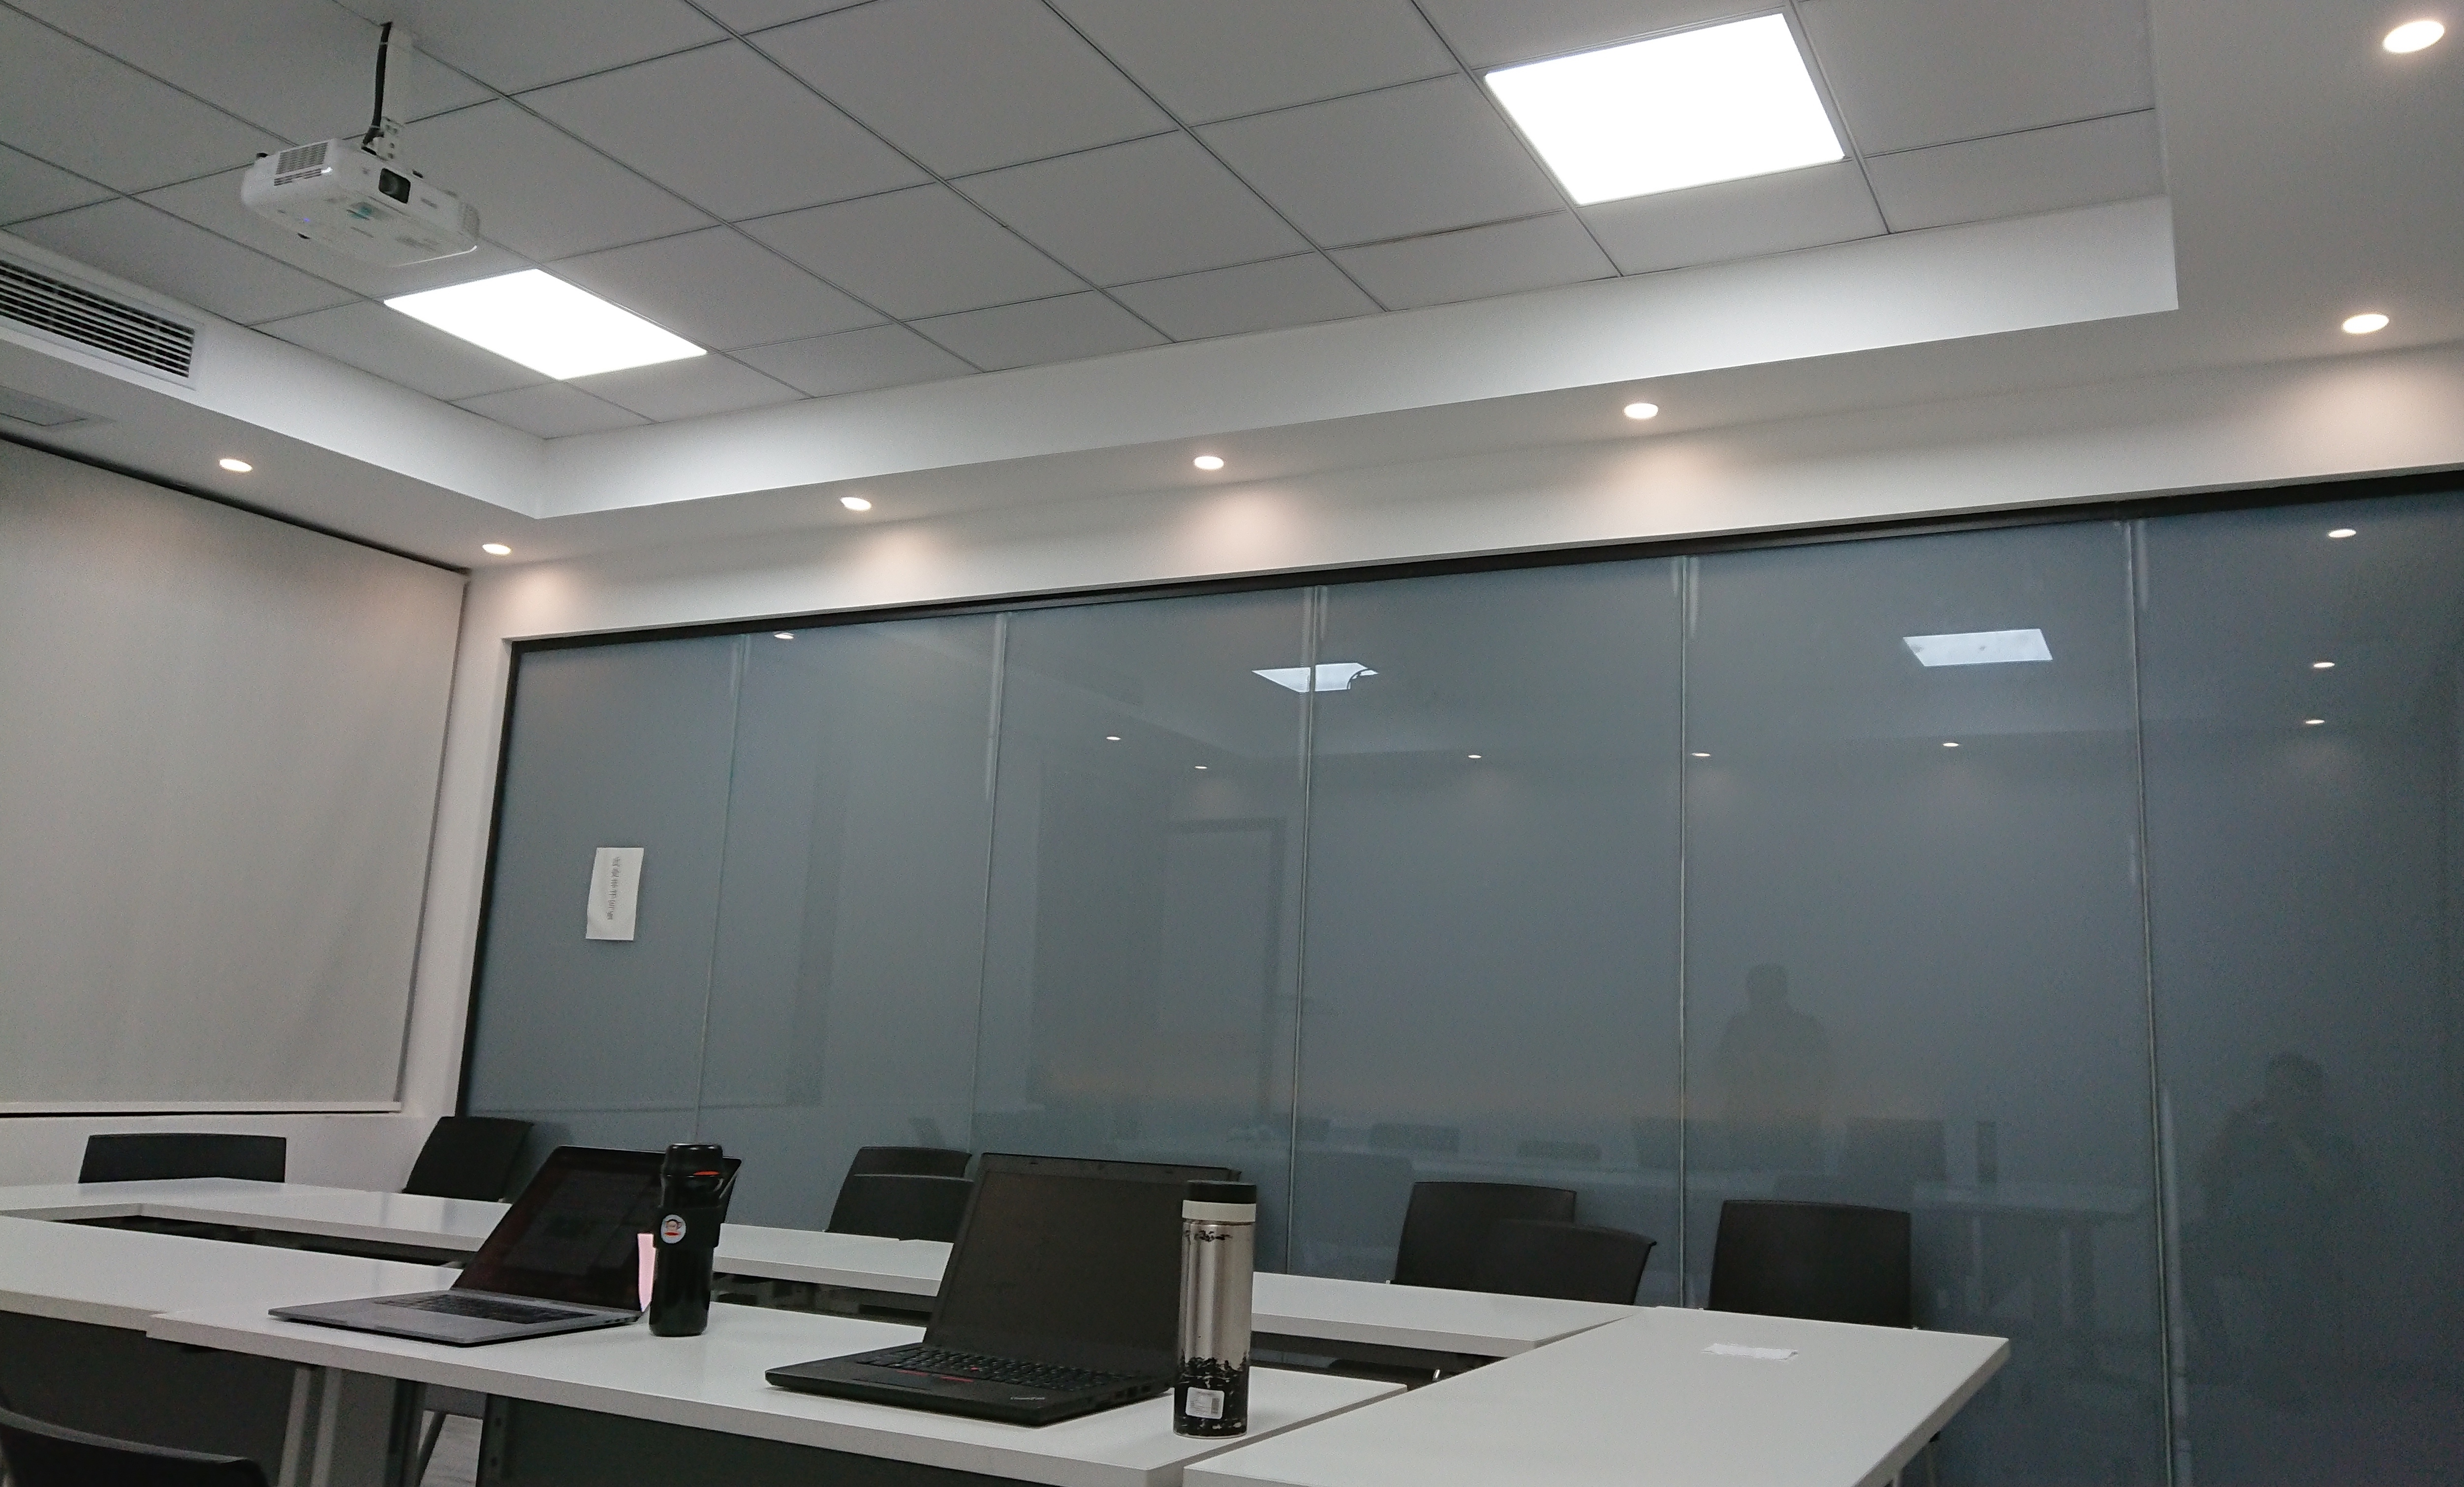
\includegraphics[width=1\linewidth]{video1}
		\caption{}
	\end{subfigure}
	\begin{subfigure}{.49\linewidth}
		\includegraphics[width=1\linewidth]{video2.jpg}
		\caption{}
	\end{subfigure}
	\caption{部分实验环境截图}\label{fig:videos}
\end{figure}

\subsection{双相目标识别实验}

\textbf{地图构建}:
在为环境构建地图的过程中,我们首先过滤绑定到非常少地图点的对象。
这是因为地图点的数量直接影响识别性能。在\autoref{table:mps}中本文列出了保留和过滤的对象,我们可以看到过滤后的对象通常尺寸较小或没有丰富的视觉特征,这符合ORB-SLAM2\cite{mur2017orb}的地图点选择方法的原则。
最后,本文选择了20个对象作为交互目标,包括13个可连接对象和7个不可连接对象。

\begin{table}[htbp]
	% \small  
	\caption{各类对象所提取的特征点数量(部分)}  \label{table:mps} 
	\begin{center}  
		\begin{tabular}{|l|l|l|l| p{4cm}|}  
			\hline  
			\textbf{被过滤对象} & \textbf{地图点数量} & \textbf{保留的对象} & \textbf{地图点数量}\\ \hline  
			box & 15 & PC & 355  \\ \hline 
			chair & 13 & table & 239  \\ \hline 
			chair & 9 & display & 83  \\ \hline  
			chair & 22 & Paper cutter & 226  \\ \hline  
			box & 43 & printer & 291  \\ \hline  
			chair & 9 & water fountain & 216  \\ \hline  
		\end{tabular}  
	\end{center}  
\end{table} 

\textbf{系统延迟}:
本文将对象识别的VSLink延迟数据与其他方法进行了比较。考虑了两种方法。一种是SnapLink\cite{chen2018snaplink}采用的基于图像定位的方法,另一种是将目标检测神经网络与图像检索相结合。本文用于比较的神经网络是原始的YOLOv5s\cite{glenn_jocher_2020_4154370},没有进行稀疏卷积的修改。

\begin{figure}[htbp]
	\centering
	\includegraphics[width=0.65\linewidth]{latency_all.pdf}
	\caption{系统延迟对比}
	\label{fig:latency comparison}
\end{figure}

我们在同一台机器上对四个视频运行了20次这些算法,结果显示在\autoref{fig:latency comparison}中。
首先,我们可以看到,对于那些稳定的对象,VSLink可以在20毫秒内检测到它们的存在,这与ORBSLAM的运行频率一致。在这个过程中,VSLink不需要计算视觉特征,而是重用SLAM结果。
然而,其他两种方法需要更多的时间进行特征计算,即100ms以上。
然后,对于可移动对象,SnapLink无法处理这种情况,因为场景与数据库中的图像不匹配,而对于神经网络,其花费的时间与稳定对象相同,大于100ms。
VSLink平均需要76毫秒左右才能完成加速推理。然而,这不是每个帧都需要的,因为\cite{yao2020video}已经提出了基于帧变化选择性执行对象检测的方法。
因此,VSLink的整个平均处理时间在33ms以下。
虽然原始的YOLOv5s方法不需要等待其他过程,但它完成推断需要120毫秒。
 
总而言之,VSLink可以支持每秒30帧的视频流,用于多对象识别,并且在速度上优于其他两种方法$4$倍。

\begin{figure}[htbp]
	\centering
	\includegraphics[width=0.65\linewidth]{NN1.pdf}
	\caption{使用子图后目标检测延迟的改善}
	\label{fig:latency improvement}
\end{figure}

\textbf{稀疏推理加速}:
本文采用高性能的目标检测神经网络YOLO\cite{redmon2016you}来评估本文提出的推理加速方法。
本文选择了不同尺寸和结构的模型,分别为YOLOv5s、YOLOv5m、YOLOv5l和YOLOv3,其中s, m, l表示模型尺寸。
所有神经网络都在Pytorch中训练,并使用TorchScript导出。导出之后,可以在C++环境中调用它们。
在\autoref{fig:latency improvement}中,本文通过引入可忽略区域和稀疏卷积来显示神经网络的延迟减少。这表明所有的神经网络都有延迟下降。YOLOv5s、YOLOv5m和YOLOv5L的速度提升分别为33.1\%、34.4\%和37.0\%。
我们认为更大的模型会得到更好的速度提升。

在实验中,我们对YOLO系列模型进行了测试。
然而,YOLO系列只是目标检测神经网络的一种类型。
我们认为,只要网络中包含卷积块,理论上所有的目标检测神经网络都将受益于这种推理加速。对于其他类型的神经网络,只是加速程度会有所不同。
例如,已知Faster R-CNN是两阶段的模型,因此对它进行加速的过程会不同于一阶段的模型。
两阶段模型首先使用RPN生成包围盒,然后使用分类模型生成对象标签。由于涉及到完全连接层,我们需要在一阶段之后再对输入进行修改。


\begin{figure*}[htbp]
	\centering
	\includegraphics[width=0.95\linewidth]{ident-res}
	\caption{使用子图后目标检测准确率的改善}
	\label{fig:identification}
\end{figure*}

\textbf{VSLink的识别准确率}:
我们计算了VSLink的识别准确率,并将结果绘制在\autoref{fig:identification}中。我们可以看到,双相识别平均准确率达到72.7\%。对于基于SLAM匹配的方法,平均准确率为49.2\%,而对于只基于神经网络的方法,平均准确率为44.7\%。这两种方法互为补充,实现了多目标识别。在这里,我们没有针对本文的实验场景对神经网络进行再训练,因为我们希望它是通用的,并且我们认为在使用专门重训练过的神经网络时它应该会表现出更好的性能。

我们认为漏检可分为两种情况:
一是我们在SLAM匹配和神经网络检测方面都失败了,所以我们需要考虑1)训练更好的神经网络,2)优化地图构建过程,让这个对象产生更多的地图点。
二是小物体无法被VSLink所捕捉。非常小的物体如\autoref{fig:small}中左端的插头对于VSLink来说是极大的挑战,因为它们既没有较多特征点,也不容易被神经网络检测到。
我们希望通过神经网络的改进提高对小目标检测的能力,学术界对此正在进行研究,并且取得了一定进展。
\begin{figure}[htbp]
	\centering
	\includegraphics[width=0.65\linewidth]{small.jpg}
	\caption{小物体的特征点}
	\label{fig:small}
\end{figure}

\textbf{移动物体的识别}:
对于第四次/第五次视频,我们手动移动了六个对象,包括三个小范围移动的对象和三个大范围移动的对象。
对于小范围移动的对象,我们将它们移动了一小段距离(小于50厘米)。对于大范围移动的物体,我们将它们移动了很长的距离(超过2米)。
我们测试了VSLink是否可以重新识别移动的对象。
结果表明,该方法对小范围移动物体的识别准确率为83\%,对大范围移动物体的识别准确率为66\%。
由于本文依靠神经网络进行可移动目标的检测,如果需要提高可移动物体的识别率,需要我们采用更先进、更精确的网络。


\textbf{鲁棒性}:
我们通过五天的使用评估了VSLink的鲁棒性。在第四天和第五天,我们在环境中手动移动了一些对象。
实验结果显示,在最后一天,对象识别的准确率下降了10\%。我们分析了实验数据,发现基于SLAM匹配的识别在不同的光照条件或环境变化时出现了更多的未匹配点。这意味着我们需要随着时间的推移主动更新地图,否则地图会随时间流逝而逐渐失效。
而时间因素通常不会影响基于神经网络的检测的鲁棒性。

% 在我们的实现中,我们还没有实现地图实时更新的方法,但我们认为这是可行的。地图实时更新面临的挑战是主动更新地图点并对其进行标记,这需要执行实例分割神经网络,并且需要花费大量时间。
% 我们可以让我们的主线程,即双相目标识别过程,占用主要的计算资源。
% 地图更新线程以延后的方式执行。


\subsection{交互定制实验}

\begin{figure*}[htbp]
	\centering
	\includegraphics[width=0.95\linewidth]{UIdesign}
	\caption{UI定制页面}
	\label{fig:ui}
\end{figure*}

为了评估VSLink如何实现灵活的用户交互定制,我们进行了一项用户调研。在用户调研中,我们为参与者提供了一份详细的按步骤进行指导操作的用户手册,以指导他们使用VSLink设计由自己定制的UI。UI设计过程通过Web应用程序实现,如\autoref{fig:ui}中所示。图中的页面左边是UI库,中间是用于定制的画布,左边是UI的文档。

\textbf{用户调研中的开发者}: 
我们在学校招募了十名志愿者,其中包括五名博士生和五名硕士生。他们中的大多数人几乎都没有UI设计经验。我们要求每位志愿者通过VSLink实现两台设备的UI。我们在实验中收集了各个重要步骤的完成时间戳并分析了数据。


\begin{table}[htbp]
    \caption{用户调研量化结果}
	\label{table:feedback_quant}
	\begin{center}
		\begin{tabular}{|l|c|}
			\hline
			对象 & 平均设计时间 \\ \hline
			智能LED(无模板) & 5分钟 \\ \hline
			智能风扇(无模板) & 2分40秒 \\ \hline
			智能LED(有模板) & 31秒 \\ \hline
			智能风扇(有模板) & 1分28秒 \\ \hline
		\end{tabular}
	\end{center}
\end{table}
\textbf{量化结果}: 
首先,志愿者们被要求设计一个智能LED灯的UI,它有3个API。他们在按步骤编写的用户手册的指导下进行设计,结果表明志愿者们平均可以在五分钟内完成设计。第一个实验一般需要比正常流程更长的时间,因为志愿者需要首先学习如何使用VSLink和阅读UI文档之后才能开始正常使用。
接下来,志愿者们被要求设计一个智能风扇的UI,它有7个API,我们没有提供任何额外指导。这次设计的过程平均需要2分40秒。实验结果表明,在完成第一次实验后,后续的实验中志愿者们的设计速度大大提高。
最后,为了评估提供模板的情况下用户设计UI的速度,我们让志愿者使用VSLink提供的模板再次设计LED灯和智能风扇的UI。结果表明,以模板作为设计基础的情况下,志愿者完成LED灯和智能风扇的UI设计平均只需要31秒和1分28秒。

\textbf{志愿者反馈}:
为了获得志愿者的其他意见,我们询问了志愿者对时间成本、定制模板和页面美化的意见,最后我们获得了\autoref{table:feedback}中的意见:
% \begin{itemize}
%   \item 所有志愿者都认为时间成本是可以接受的;
%   \item 八名志愿者认为他们自己定制出来的UI比我们提供的模板更好,另外两人则认为两者没有大的区别;
%   \item 一半的志愿者认为他们设计UI的网页还有进一步改进和美化的空间。
% \end{itemize}
\begin{table}[htbp]
    \caption{志愿者反馈意见}
	\label{table:feedback}
    \begin{tabularx}{\linewidth}{|c|X|}
        \hline
        类别 & 意见 \\ \hline
        时间成本 & 所有志愿者都认为时间成本是可以接受的 \\ \hline
        定制模板 & 八名志愿者认为他们自己定制出来的UI比我们提供的模板更好,另外两人则认为两者没有大的区别 \\ \hline
        页面美化 & 一半的志愿者认为他们设计UI的网页还有进一步改进和美化的空间 \\ \hline
    \end{tabularx}
\end{table}


\section{案例验证}
为了演示VSLink在人机交互方面的能力。我们使用VSLink开发三个应用场景,如\autoref{fig:cases}所示。

\begin{figure}[htbp]
	\centering
	\begin{subfigure}{.65\linewidth}
		\includegraphics[width=1\linewidth]{case1}
		\caption{}
	\end{subfigure}
	\begin{subfigure}{.65\linewidth}
		\includegraphics[width=1\linewidth]{case2}
		\caption{}
	\end{subfigure}
	\begin{subfigure}{.65\linewidth}
		\includegraphics[width=1\linewidth]{case3}
		\caption{}
	\end{subfigure}
	\caption{三个VSLink实现的应用}\label{fig:cases}
\end{figure}

\subsection{设备管理}
第一个场景是设备管理。对于实验室中的公共设备,我们在虚拟世界中记录并显示其元数据,如该设备的设备名称与型号、该设备的设备参数、设备购入/入库时间、该设备当前归属的用户/员工等重要数据。此功能有助于公司或实验室等组织管理和维护其纷繁复杂的设备。如\autoref{fig:cases}a中,我们将手机摄像头对着显示器,即可在其上方看到该显示器的具体信息,包括显示器的名称和型号,它所支持的分辨率,购入时间和历任使用者。

除了显示设备信息,在记录了各个设备位置的情况下,此案例还可以帮助寻找已登记设备的位置,当我们需要在设备仓库的大量设备中中寻找某个特定的设备时,我们可以先在设备列表中找到该设备,并令其单独显示在虚拟世界中,随后我们即可通过手机屏幕/AR眼镜找到该设备的物理位置。
\subsection{智能会议室}
第二个场景是智能会议室。我们将VSLink连接到会议室的设备,并设计相应的UI。用户可以通过VSLink控制门、中央空调、玻璃墙、投影仪和扬声器。我们在场景中实现了以下功能:
\begin{itemize}
	\item 在进入会议室前,我们可以在网络上提前预定会议室,到会议开始前即可通过VSLink在门禁上显示的交互界面进行门禁解锁进入会议室,如\autoref{fig:meeting}a;
	\item 进入会议室后,可以通过VSLink查看中央空调当前温度和风速,并使用滚动条调节中央空调的目标温度,如\autoref{fig:meeting}b;
	\item 在会议前可以通过VSLink在座位上查看在会议室的座位安排,如\autoref{fig:meeting}c;
	\item 通过VSLink启动会议室的玻璃墙雾化,将会议室与外界封闭,如\autoref{fig:meeting}d;
	\item 通过VSLink打开投影仪,并降下投影幕布,如\autoref{fig:meeting}e;
	\item 通过VSLink调节麦克风的音量,如\autoref{fig:meeting}f。
\end{itemize}
\subsection{植物养护}
第三个场景是植物养护。对于养植物的用户,我们设计了交互功能来记录浇水时间和浇水量,并记录重要日期,如开花日,同时,我们在盆中植入了湿度传感器,以检测浇水的效果。虽然植物并没有连接到互联网,但是通过VSLink,我们为植物在虚拟空间中创建了对应的对象,并在平台中为同时将其中的一个显示组件绑定到湿度传感器。通过VSLink在植物上的应用,我们可以科学地完成植物培育。

\begin{figure}[htb]
	\centering
	\begin{subfigure}{.48\linewidth}
		\includegraphics[width=1\linewidth]{meeting1.jpg}
		\caption{}
	\end{subfigure}
	\quad
	\begin{subfigure}{.48\linewidth}
		\includegraphics[width=1\linewidth]{meeting2.jpg}
		\caption{}
	\end{subfigure}
	\quad
	\begin{subfigure}{.48\linewidth}
		\includegraphics[width=1\linewidth]{meeting3.jpg}
		\caption{}
	\end{subfigure}
	\quad
	\begin{subfigure}{.48\linewidth}
		\includegraphics[width=1\linewidth]{meeting4.jpg}
		\caption{}
	\end{subfigure}
	\quad
	\begin{subfigure}{.48\linewidth}
		\includegraphics[width=1\linewidth]{meeting5.jpg}
		\caption{}
	\end{subfigure}
	\quad
	\begin{subfigure}{.48\linewidth}
		\includegraphics[width=1\linewidth]{meeting6.jpg}
		\caption{}
	\end{subfigure}
	\caption{智能会议室案例}\label{fig:meeting}
\end{figure}

\section{本章小结}
这一章节我们描述了VSLink的系统实现并展示了VSLink的实验评估结果:

1. 描述了VSLink的系统架构和具体实现细节;

2. 描述了实验设置,对系统的延迟表现、稀疏推理的加速效果以及VSLink的识别准确率进行了实验,并评估了VSLink的鲁棒性。

3. 我们完成了VSLink的交互定制实验,以用户调研的方式对用户体验进行了调查。

4. 我们还为VSLink实现了三个应用场景示例,探索VSLink能够实现的可能性。

\chapter{总结与展望}
\label{chap:sum}
\section{研究总结}
在本文中,我们提出了VSLink,这是一种基于增强现实的人机交互解决方案,依靠视觉SLAM定位和神经网络实现目标的识别和定位,使用稀疏推理加速神经网络计算,结合用户可自由定制的交互平台,实现了实时视频流下与环境对象的快速和普适交互。本文的主要创新点总结如下:

1.本文提出了一种双相目标识别方法来快速准确地识别和定位目标,使用VSLAM对目标进行精准的定位,并使用目标检测神经网络对目标进行识别;

2.本文提出了SLAM与神经网络结合的网络推理加速方法,基于VSLAM提供的可忽略区域,屏蔽已识别对象的区域,利用稀疏推理进行神经网络推理的加速,以降低推理的延迟;

3.本文设计了一个交互平台来实现高度可定制的交互,基于物模型的设备抽象和已有的物联网设备平台,为各类设备提供了一个交互组件库,以Web技术实现无代码的交互界面设计,为用户提供高度可定制的交互体验;

4.本文基于边缘计算架构实现了VSLink,并在包含多个对象并且对象可移动的环境中对其进行了评估。结果表明,VSLink支持30FPS视频输入,实现了实时运行,并且目标识别率达到了{\acc}。我们在三个典型场景对VSLink进行了案例验证,结果表明VSLink在各类场景下都可以为用户提供所见即所得的良好交互体验。

\section{未来工作}
基于本文已完成的工作和存在的不足,未来还可以在以下方面进行研究工作:
\begin{itemize}
	\item 可以将深度神经网络进一步与视觉SLAM进行结合,统一神经网络和SLAM的特征提取,共享图像特征信息,深度融合SLAM与目标识别神经网络,提高识别率和识别速度,进一步节约计算资源;
	\item 进一步探索各类设备的抽象方式和类别,并设计针对性的DSL(Domain Specific Language)用于对设备的模型和设备交互行为进行描述,以实现简化的设备逻辑描述,方便用户定制设备的运行逻辑;
	\item 增加虚拟传感器层,用神经网络或者用户定义的逻辑,以其他实体传感器或来自互联网的信息为数据源,推理生成用户所需的信息,形成虚拟传感器,充分利用各类数据和神经网络的推理能力增强交互的智能程度。
	\item 探索神经网络视频事件识别在增强现实中的应用,以允许进一步的设备智能化,平台可以依靠摄像头所拍摄的视频流自动推断现实世界的事件,结合平台的设备信息,根据设定的逻辑完成对应的设备操作;
	\item 探索自动化的逻辑生成,根据平台识别出的事件序列和用户操作序列,结合神经网络和知识图谱等技术自动学习各类事件和操作中潜在的运行逻辑,以推送给用户的方式或自动生效的方式提高家居/工厂/办公智能化。
\end{itemize}
% \chapter{参考命令}
% \section{节标题}

% 我们可以用includegraphics来插入现有的jpg等格式的图片,
% 如\autoref{fig:zju-logo}所示。

% \begin{figure}[htbp]
%     \centering
%     \includegraphics[width=.3\linewidth]{logo/zju}
%     \caption{\label{fig:zju-logo}浙江大学LOGO}
% \end{figure}


% \subsection{小节标题}


% \par 如\autoref{tab:sample}所示,这是一张自动调节列宽的表格。

% \begin{table}[htbp]
%     \caption{\label{tab:sample}自动调节列宽的表格}
%     \begin{tabularx}{\linewidth}{c|X<{\centering}}
%         \hline
%         第一列 & 第二列 \\ \hline
%         xxx & xxx \\ \hline
%         xxx & xxx \\ \hline
%         xxx & xxx \\ \hline
%     \end{tabularx}
% \end{table}


% \par 如\autoref{equ:sample},这是一个公式

% \begin{equation}
%     \label{equ:sample}
%     A=\overbrace{(a+b+c)+\underbrace{i(d+e+f)}_{\text{虚数}}}^{\text{复数}}
% \end{equation}

% \chapter{另一章}

% \begin{figure}[htbp]
%     \centering
%     \includegraphics[width=.3\linewidth]{example-image-a}
%     \caption{\label{fig:fig-placeholder}图片占位符}
% \end{figure}